\documentclass[acmtog]{acmart}
\usepackage{graphicx}
\usepackage{subfigure}
\usepackage{natbib}
\usepackage{listings}
\usepackage{bm}
\usepackage{amsmath}

\definecolor{blve}{rgb}{0.3372549 , 0.61176471, 0.83921569}
\definecolor{gr33n}{rgb}{0.29019608, 0.7372549, 0.64705882}
\makeatletter
\lst@InstallKeywords k{class}{classstyle}\slshape{classstyle}{}ld
%\makeatother
\lstset{language=C++,
    breaklines=true,
%    basicstyle=\ttfamily,
    keywordstyle=\color{blve}\ttfamily,
    stringstyle=\color{red}\ttfamily,
    commentstyle=\color{magenta}\ttfamily,
    morecomment=[l][\color{magenta}]{\#},
    classstyle = \bfseries\color{gr33n},
    tabsize=2,
    morekeywords={Vec3f, Interaction},
}
%\lstset{basicstyle=\ttfamily}


% Title portion
\title{Multi-Resolution Isosurface Rendering}

\author{Name:\quad Bingnan Li \quad Suting Chen \\ student number:\ 2020533092\ 2020533185
\\email:\quad libn@shanghaitech.edu.cn\quad chenst@shanghaitech.edu.cn}

% Document starts
\begin{document}
    \maketitle

    \vspace*{2 ex}


    \section{Related Paper Overview}\label{sec:related-paper-overview}


    \section{Introduction}\label{sec:introduction}
    \begin{itemize}
        \item data preprocessing
        \item k-d tree
        \item transfer function
        \item volume rendering
        \item object rendering and object filtering
    \end{itemize}


    \section{Implementation Details}\label{sec:implementation-details}

    \subsection{data preprocessing}\label{subsec:data-preprocessing}
    In this project, we dealt with \emph{.vdb} files and try to visualize four different multi-resolution grids.
    In order to accomplish that, we utilized \emph{openvdb} library to read the \emph{.vdb} files and extract the grids.F
    Given that the vdb grids are actually velocity field around a sphere which is a vector field, we need to perform scalarization:
    \begin{enumerate}
        \item Turn the velocity field into a scalar field by using the magnitude of the velocity field.
        \item Calculate the q-criteria of the velocity field.
        \par Q-criteria is a scalar field that is used to determine the quality of the flow.
        It is defined as:
        \begin{equation}
            Q = -\frac{1}{2}\left( \left( \frac{\partial u}{\partial x} \right)^2 + \left( \frac{\partial v}{\partial y} \right)^2 + \left( \frac{\partial w}{\partial z} \right)^2 \right) - \frac{\partial u}{\partial y}\frac{\partial v}{\partial x} - \frac{\partial u}{\partial z}\frac{\partial w}{\partial x} - \frac{\partial v}{\partial z}\frac{\partial w}{\partial y}\label{eq:equation}
        \end{equation}
        where $u$, $v$, $w$ are the velocity components in the $x$, $y$, $z$ directions respectively.
        \par As for calculating the gradient, we use the \emph{Central Finite Difference Approximations}, which defines as follows:
        \begin{align*}
            f'(x)=\frac{f(x+h)-f(x-h)}{2h}
        \end{align*}
        with ths approximation, we can efficiently calculate the q-criteria from a discrete velocity field.
        \par Moreover, q-criteria field has a property that the gradient always points to the interior of the flow, which is useful when designing the transfer function.
    \end{enumerate}

    \subsection{k-d tree}\label{subsec:k-d-tree}

    \subsection{transfer function}\label{subsec:transfer-function}
    In this project, we use different scalar field to map scalar to color and opacity.
    For opacity, we use q-criteria as the input of transfer function.
    Next, we will show the detail of opacity transfer function:
    Assume that we want to visualize the q-criteria with iso-value $i$, then we set opacity as follows:
    \begin{align*}
        opacity = \left\{
        \begin{aligned}
            1&\quad if\ q \geq i\\
            0&\quad elsewhere
        \end{aligned}
        \right.
    \end{align*}
    The reason why we can simply set opacity above has been mentioned in~\ref{subsec:data-preprocessing}, since the gradient of q-criteria field always points to the interior of the iso-surface, we know that the iso-value of interior side is always larger than the exterior side.
    Based on that, if we use \emph{front-to-back} algorithm to perform volume rendering and apply \emph{early termination} like
    \begin{lstlisting}[label={lst:lstlisting}]
        if (src_opacity > 1 - 1e-2) break;
    \end{lstlisting}
    we can guarantee the correctness of the rendering result and in the meanwhile, achieve efficiency.

    For color, we use module of velocity field as the input of transfer function.
    We perform a linear interpolation between four colors with the following procedure:

    We first divided the range of the module of velocity field into four parts, and then we set the color of each part as follows:

    Assume we are in part $[m_0, m_1]$ and get module $m$, and the corresponding color of $m_0,m_1$ are $c_0, c_1$ resp.~ then the the corresponding color of $m$ is
    \[c=\frac{m_1-m}{m_1-m_0}\times c_0 + \frac{m-m_0}{m_1-m_0}\times c_1\]

    \subsection{volume rendering}\label{subsec:volume-rendering}
    For the volume rendering part, we use \emph{front-to-back} algorithm to rendering the turbulence.
    The procedure of \emph{front-to-back} algorithm is as follows:
    \begin{itemize}
        \item Initialize destination opacity and destination color to 0.
        \item Marching \emph{step\_size} length along the ray and get the source opacity and color.
        \item Accumulate opacity and color with the following formulas:
        \begin{align*}
            C_{dst} &= C_{dst} + (1-\alpha_{dst}) \times C_{src}\\
            \alpha_{dst} &= \alpha_{dst} + (1-\alpha_{dst})\times \alpha_{src}
        \end{align*}
        where $C_{dst}, C_{src}$ are the color of destination and source resp.~ and $\alpha_{dst}, \alpha_{src}$ are the opacity of destination and source resp.
        \item Once we march beyond limit or the source opacity $> 0.99$ , we terminate.
    \end{itemize}
    We attached the code:
    \begin{lstlisting}[label={lst:lstlisting2}]
float step_size = scene->grids[0].dx / 16;
Vec3f src_color;
float src_opacity;
auto src_t = (float) fmax(t0 - step_size, ray.t0());
Vec3f src_pos, dst_color = Vec3f{0, 0, 0};
float dst_opacity = 0;
float dx;
while (src_t < t1) {
    src_t += step_size;
    src_pos = ray(src_t);
    std::tie(src_color, src_opacity, dx) = scene->getEmissionOpacity(src_pos);
    step_size = dx / 16;
    src_opacity = (float) (1.0 - std::pow(1 - src_opacity, step_size));
    dst_color += (1 - dst_opacity) * src_color;
    dst_opacity += (1 - dst_opacity) * src_opacity;
    if (src_opacity > 1 - 1e-2) break;
}
return {dst_color, dst_opacity};
    \end{lstlisting}

    \subsection{object rendering and object filtering}\label{subsec:object-rendering-and-object-filtering}
    In this project, we use surface rendering (a.k.a.~ object rendering) to visualize the sphere that the wind passes through.
    This model is a simple phong-lighting model and ray-casting model but with slightly change in oder to match volume rendering:
    Beyond the simple phong-lighting model, we check whether the ray touches the volume part first by checking whether the destination opacity is larger than zero.

    We achieve this part by the following procedure: we first perform an object filtering by apply ray-sphere intersection to find the limit of marching depth.
    In order to achieve a acceptable result, we slightly dilated the radius of the sphere to ensure that all the volumes are covered by the sphere.
    Then for the rendering part, we applied another ray-sphere intersection but with the correct sphere radius in order to render the real size of the sphere.
    After that, we perform volume rendering with the marching depth determined during the first ray-sphere intersection.
    However, even this procedure can vanish most volumes attach to the sphere, there are still tiny pitches that levitate above the sphere.
    In order to solve those pitches, we adjust the size of bounding box so that those pitches are beyond the bounding box.

    For each pixel in the output image, we perform the following code:
    \begin{lstlisting}[label={lst:lstlisting3}]
Vec3f L(0, 0, 0);
float t0, t1, t_max = 1e10;
Vec3f phongColor(0);
Interaction interaction;
if (scene->sphere.aabb.intersect(ray, t0, t1)) {
   if (scene->dilated_sphere.intersect(ray, interaction)) {
       t_max = interaction.dist;
       if (scene->sphere.intersect(ray, interaction)) {
           phongColor = radiance(ray, interaction, Vec3f{4, 1.5, 0});
       }
   }
}
if (scene->grids[0].aabb.intersect(ray, t0, t1)) {
    auto colorOpacity = radiance(ray, t0, std::min(t1, t_max));
    L += colorOpacity.first;
    if (colorOpacity.second < 1 - 1e-3) {
        L += phongColor;
    }
} else {
    L += phongColor;
}
camera->getImage()->setPixel(dx, dy, L);
    \end{lstlisting}


    \section{Results}\label{sec:results}
    This part we will show the rendering results for different models and with different rendering configurations.

    \subsection{multi-resolution big model}\label{subsec:multi-resolution-big-model}
    \begin{figure}[H]
        \centering
        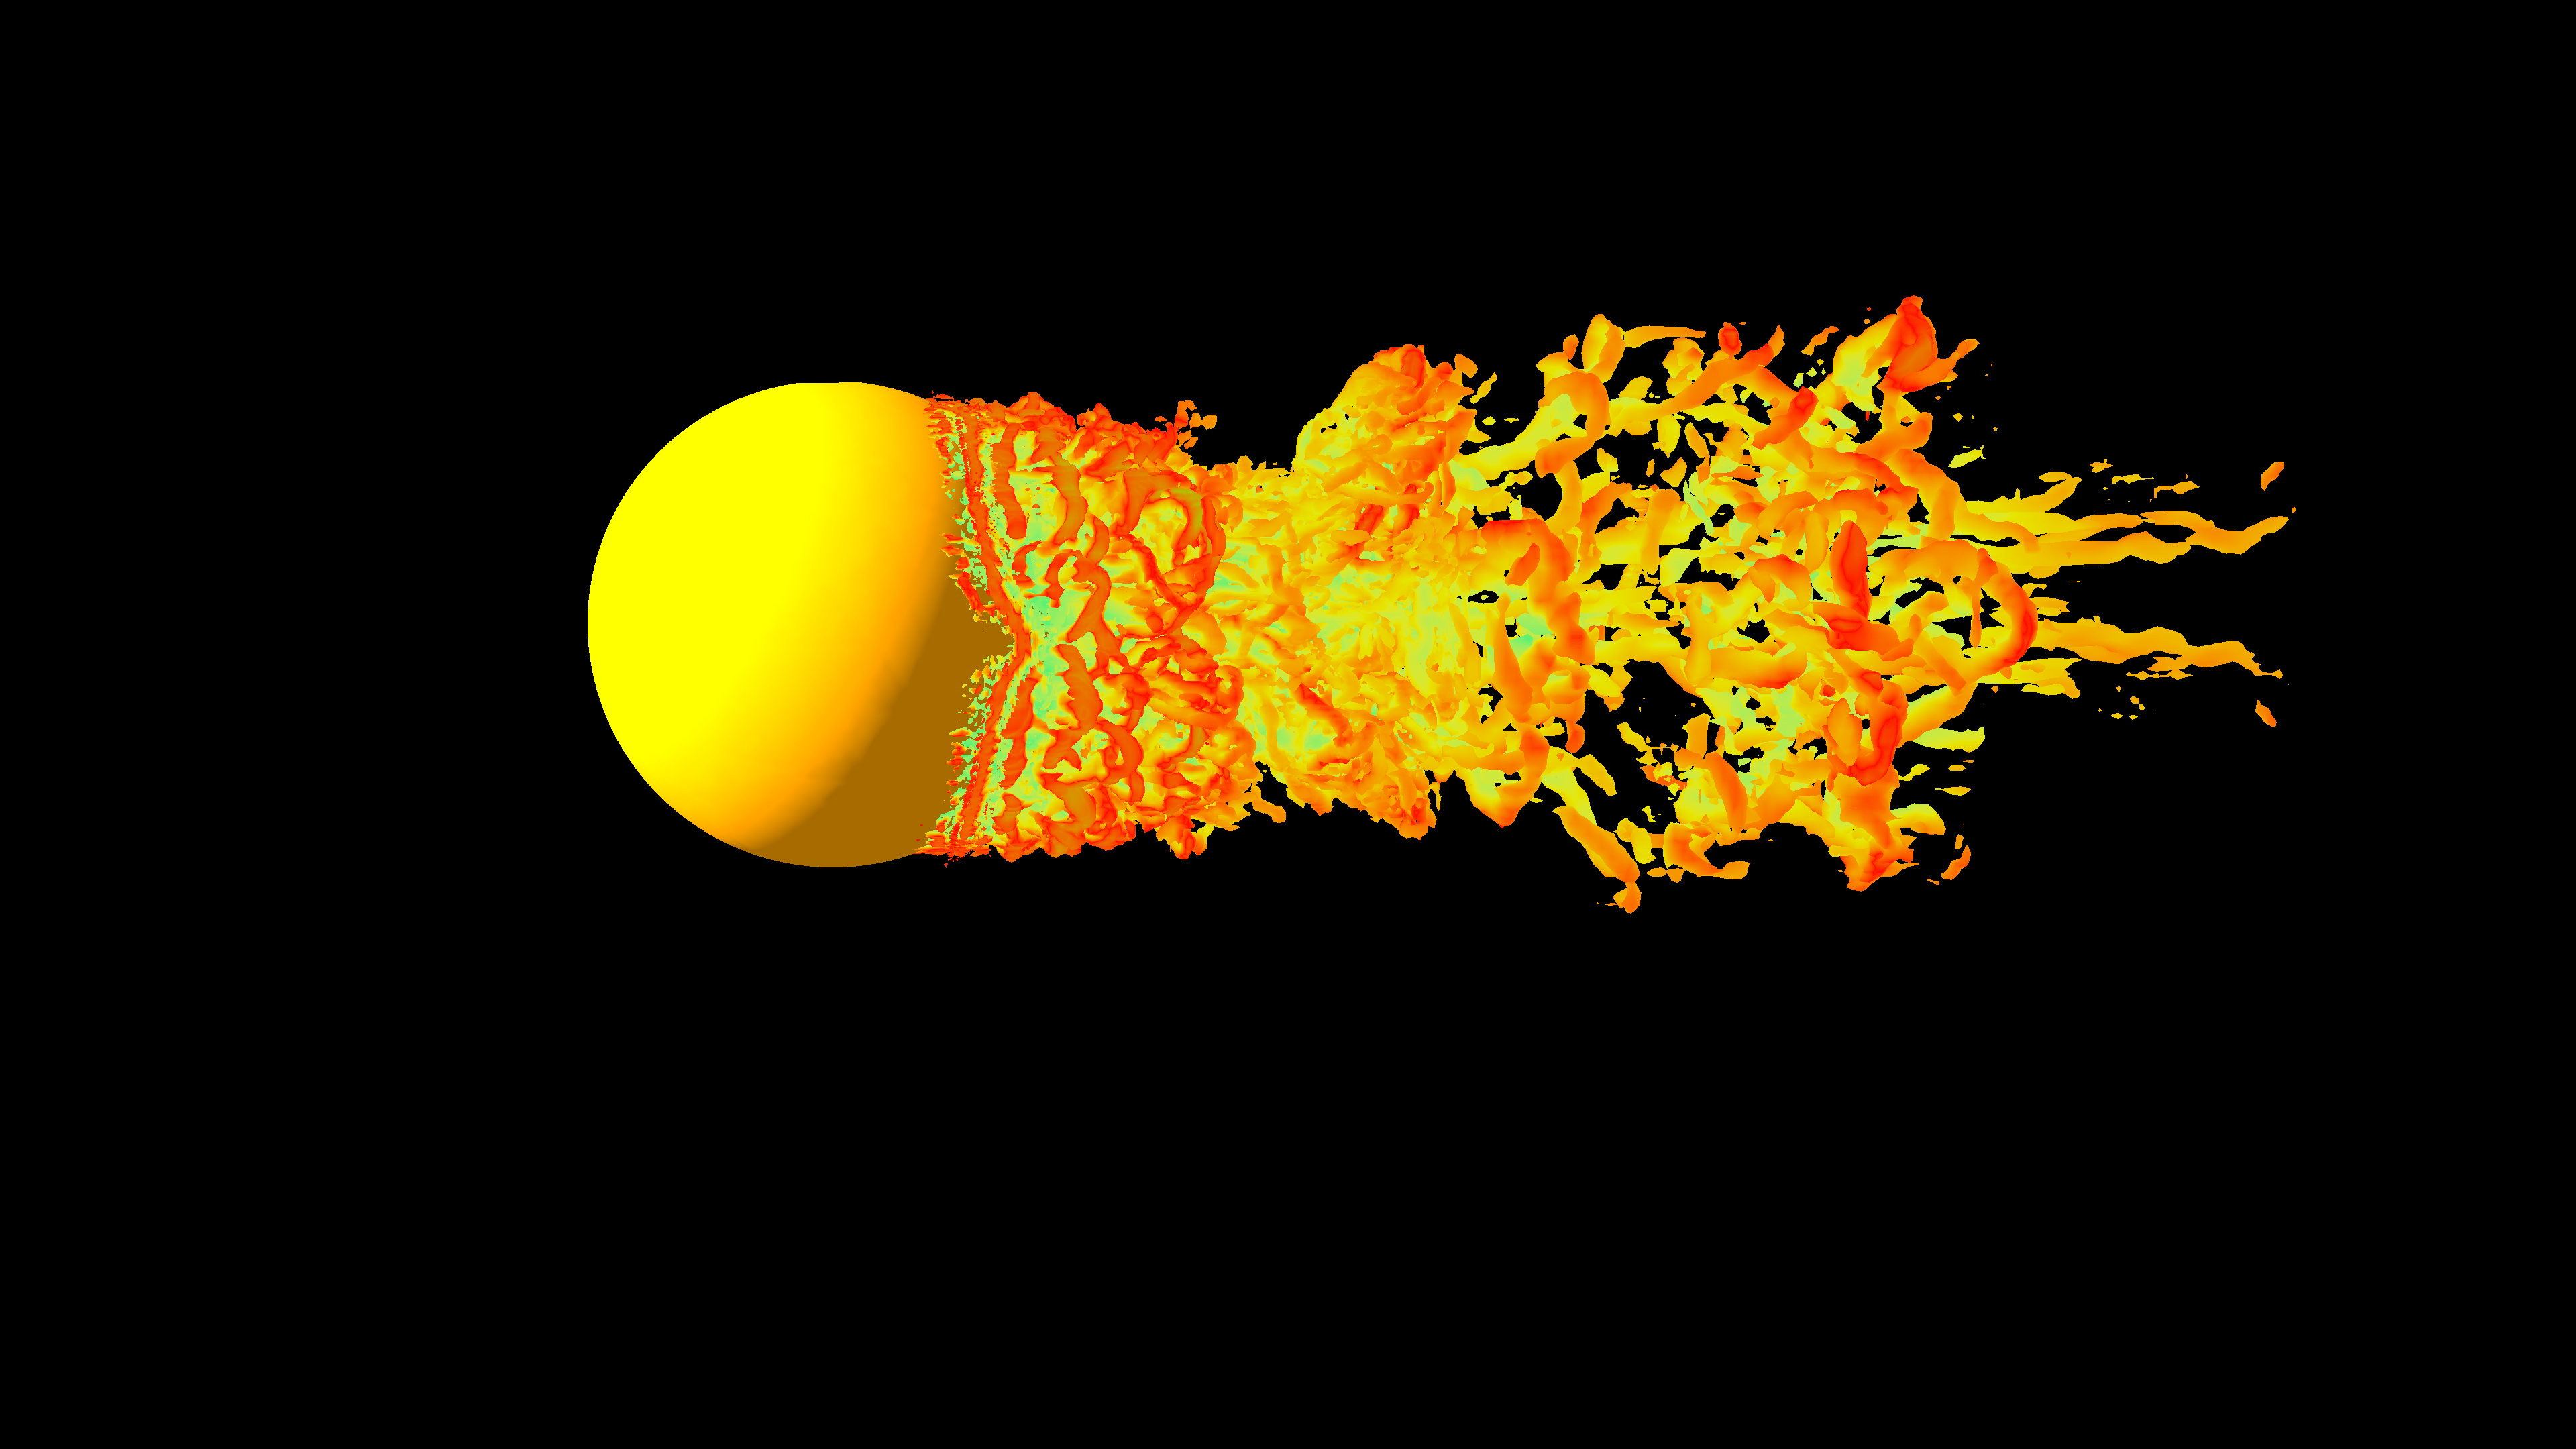
\includegraphics[width=0.45\textwidth]{./image/multi_big_4k_16_filter}
        \caption{Multi-resolution big field, 4k resolution, $ \frac{dx}{16} $ step size with object filtering (iso-value = 0.05)}\label{fig:figure1}
    \end{figure}

    \begin{figure}[H]
        \centering
        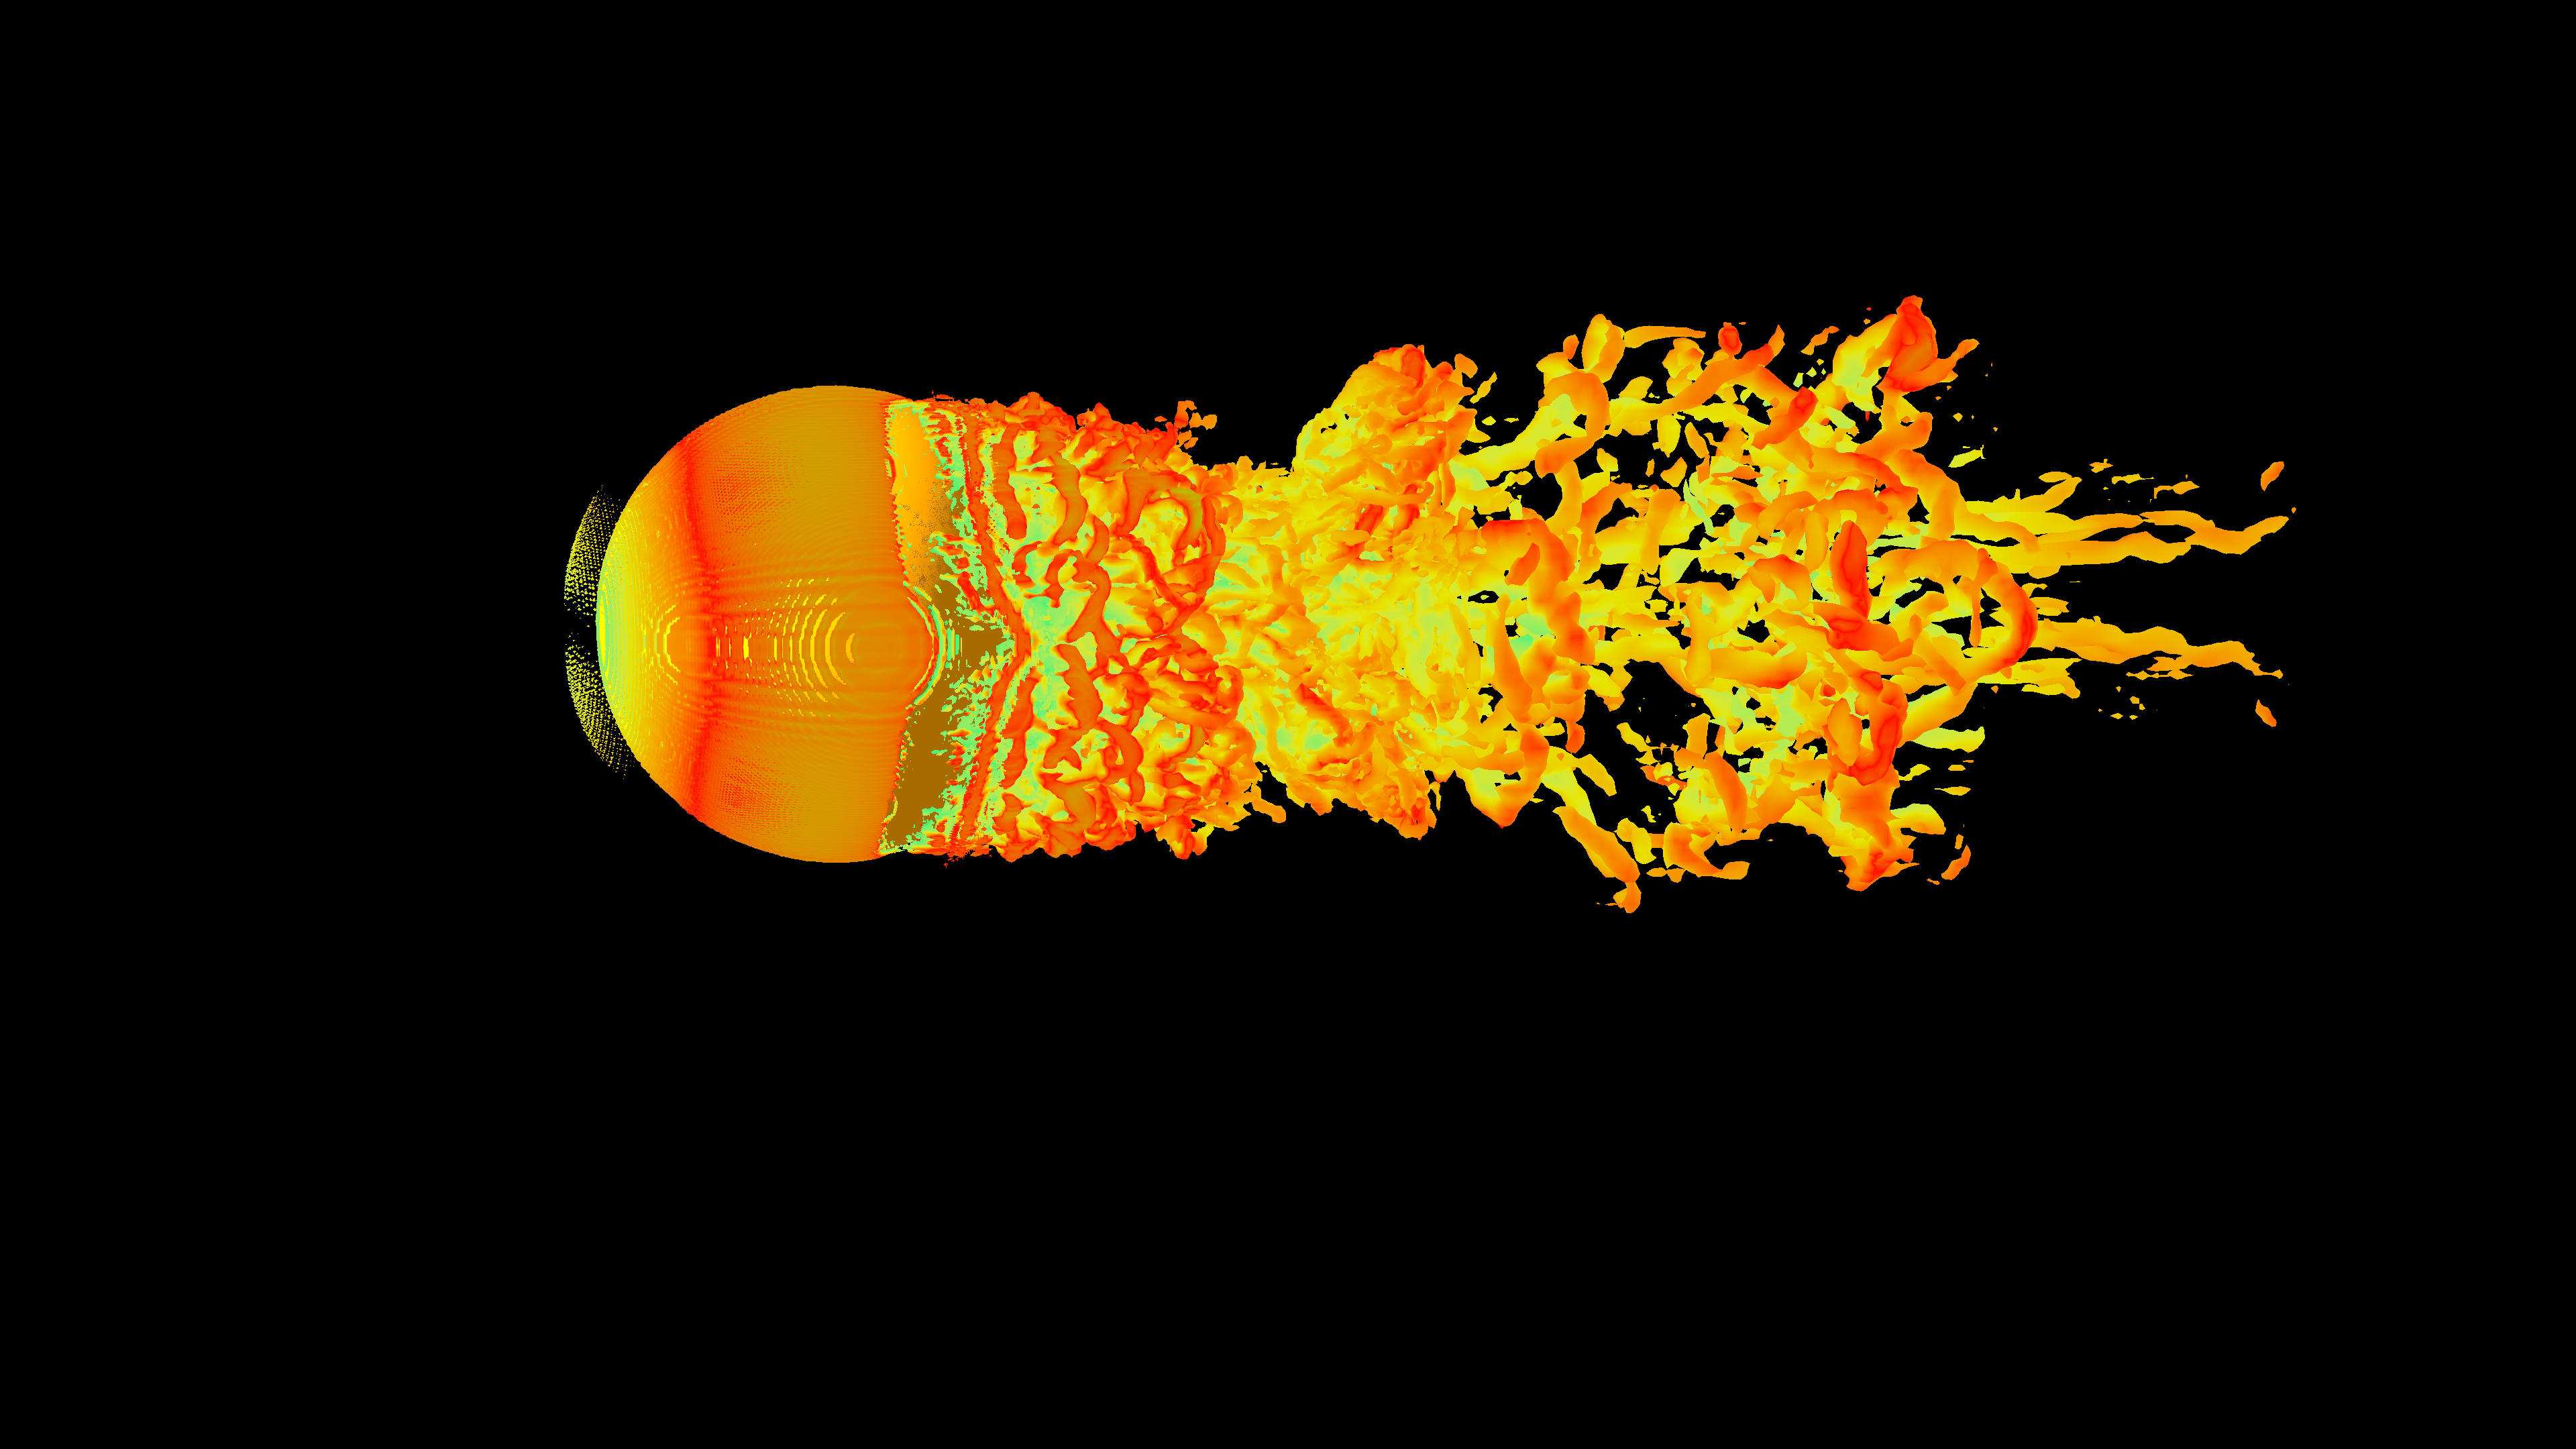
\includegraphics[width=0.45\textwidth]{./image/multi_big_4k_16_no_filter}
        \caption{Multi-resolution big field, 4k resolution, $ \frac{dx}{16} $ step size without object filtering (iso-value = 0.05)}\label{fig:figure2}
    \end{figure}

    \begin{figure}[H]
        \centering
        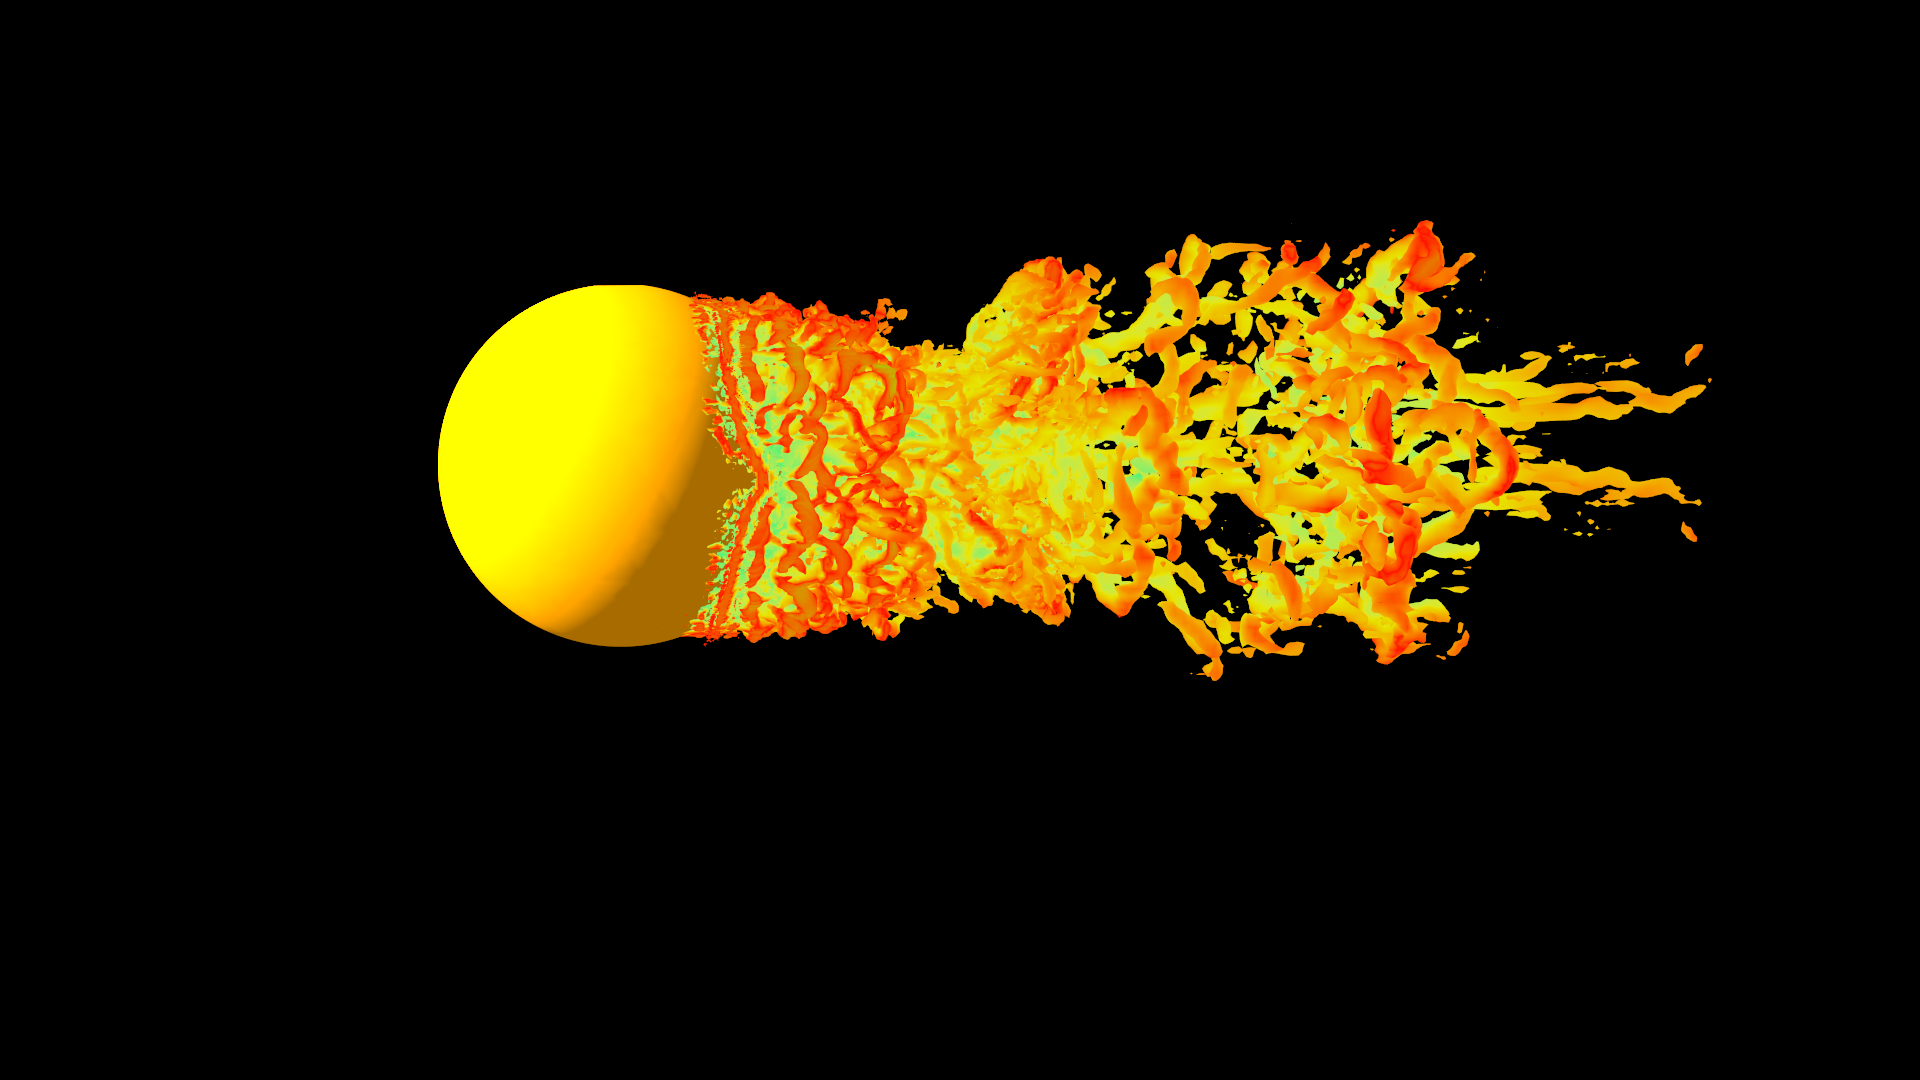
\includegraphics[width=0.45\textwidth]{./image/multi_big_1080p_8_filter_4XRES}
        \caption{Multi-resolution big field, 1080p resolution, $ \frac{dx}{8} $ step size with object filtering and 4X super resolution anti-aliasing (iso-value = 0.05)}\label{fig:figure3}
    \end{figure}

    \begin{figure}[H]
        \centering
        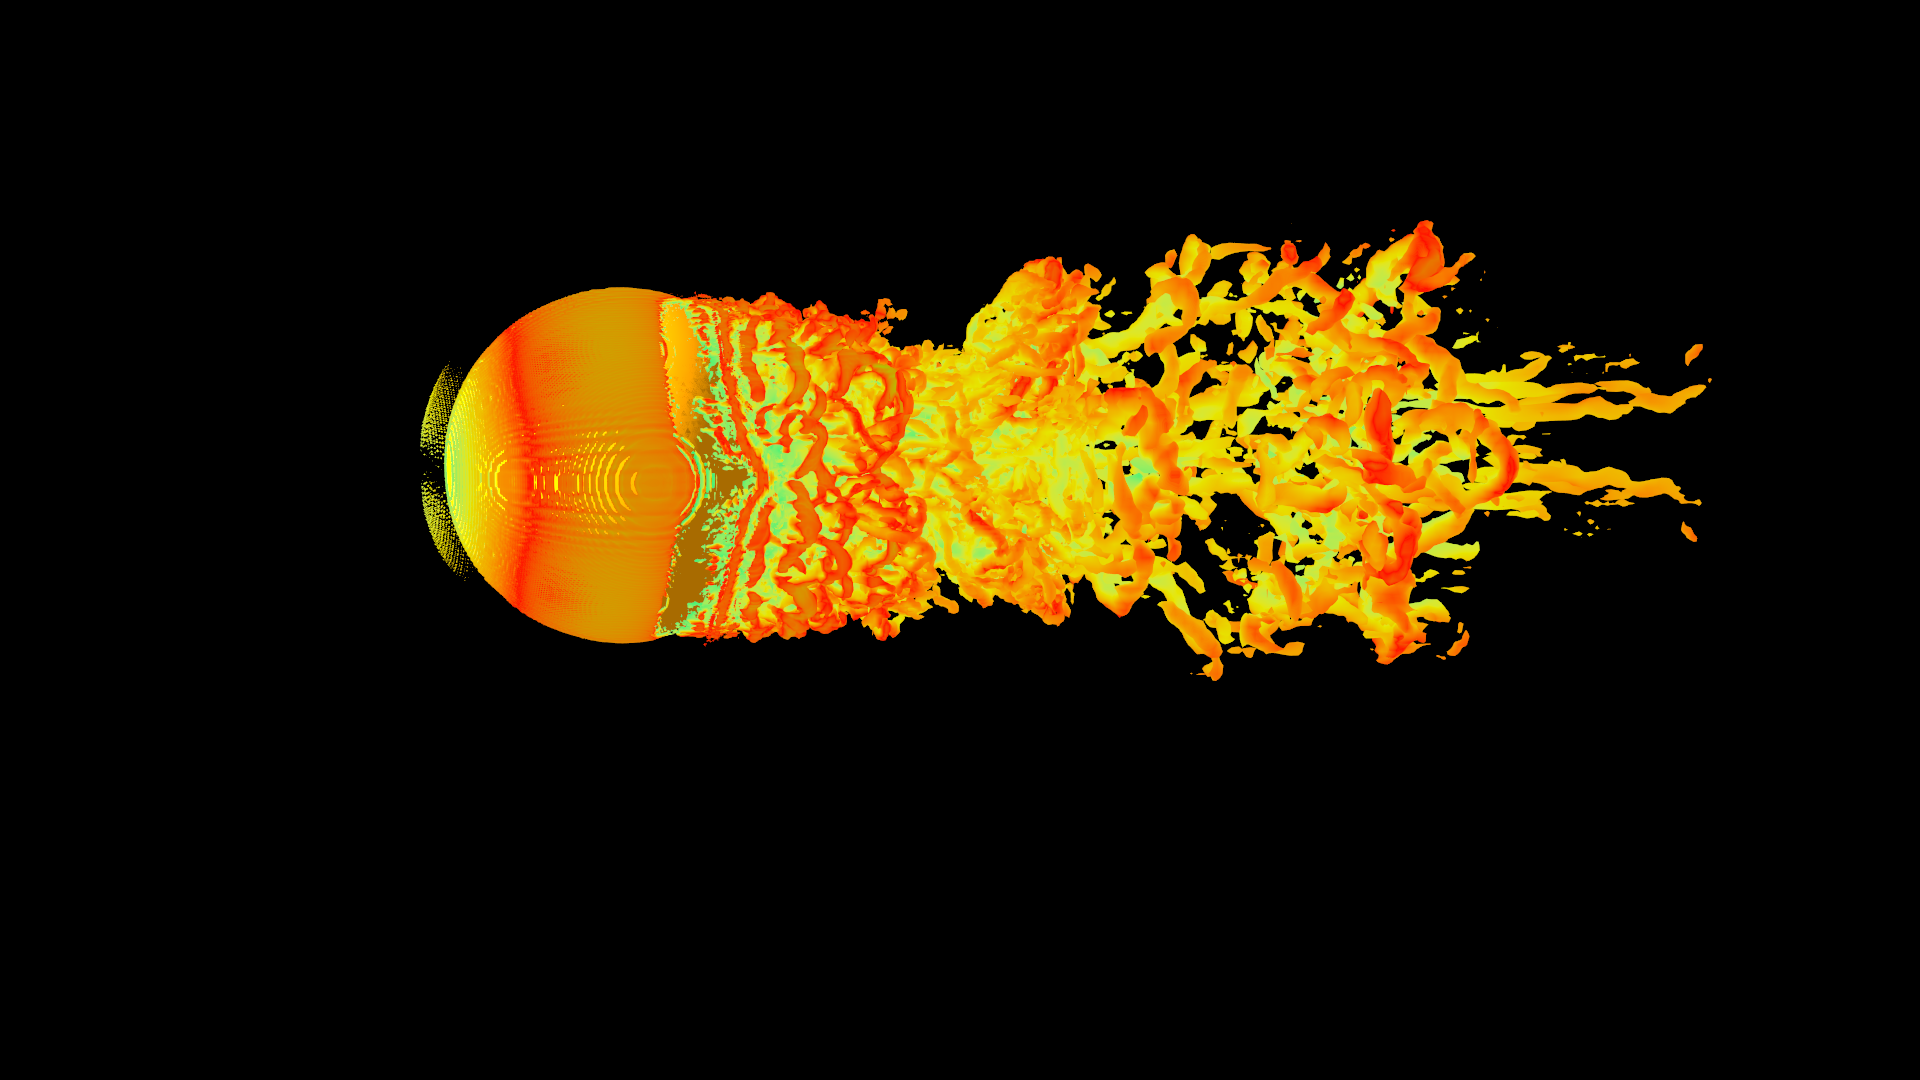
\includegraphics[width=0.45\textwidth]{./image/multi_big_1080p_8_no_filter_4XRES}
        \caption{Multi-resolution big field, 1080p resolution, $ \frac{dx}{8} $ step size without object filtering and 4X super resolution anti-aliasing  (iso-value = 0.05)}\label{fig:figure4}
    \end{figure}

    \subsection{multi-resolution small model}\label{subsec:multi-resolution-small-model}
    \begin{figure}[H]
        \centering
        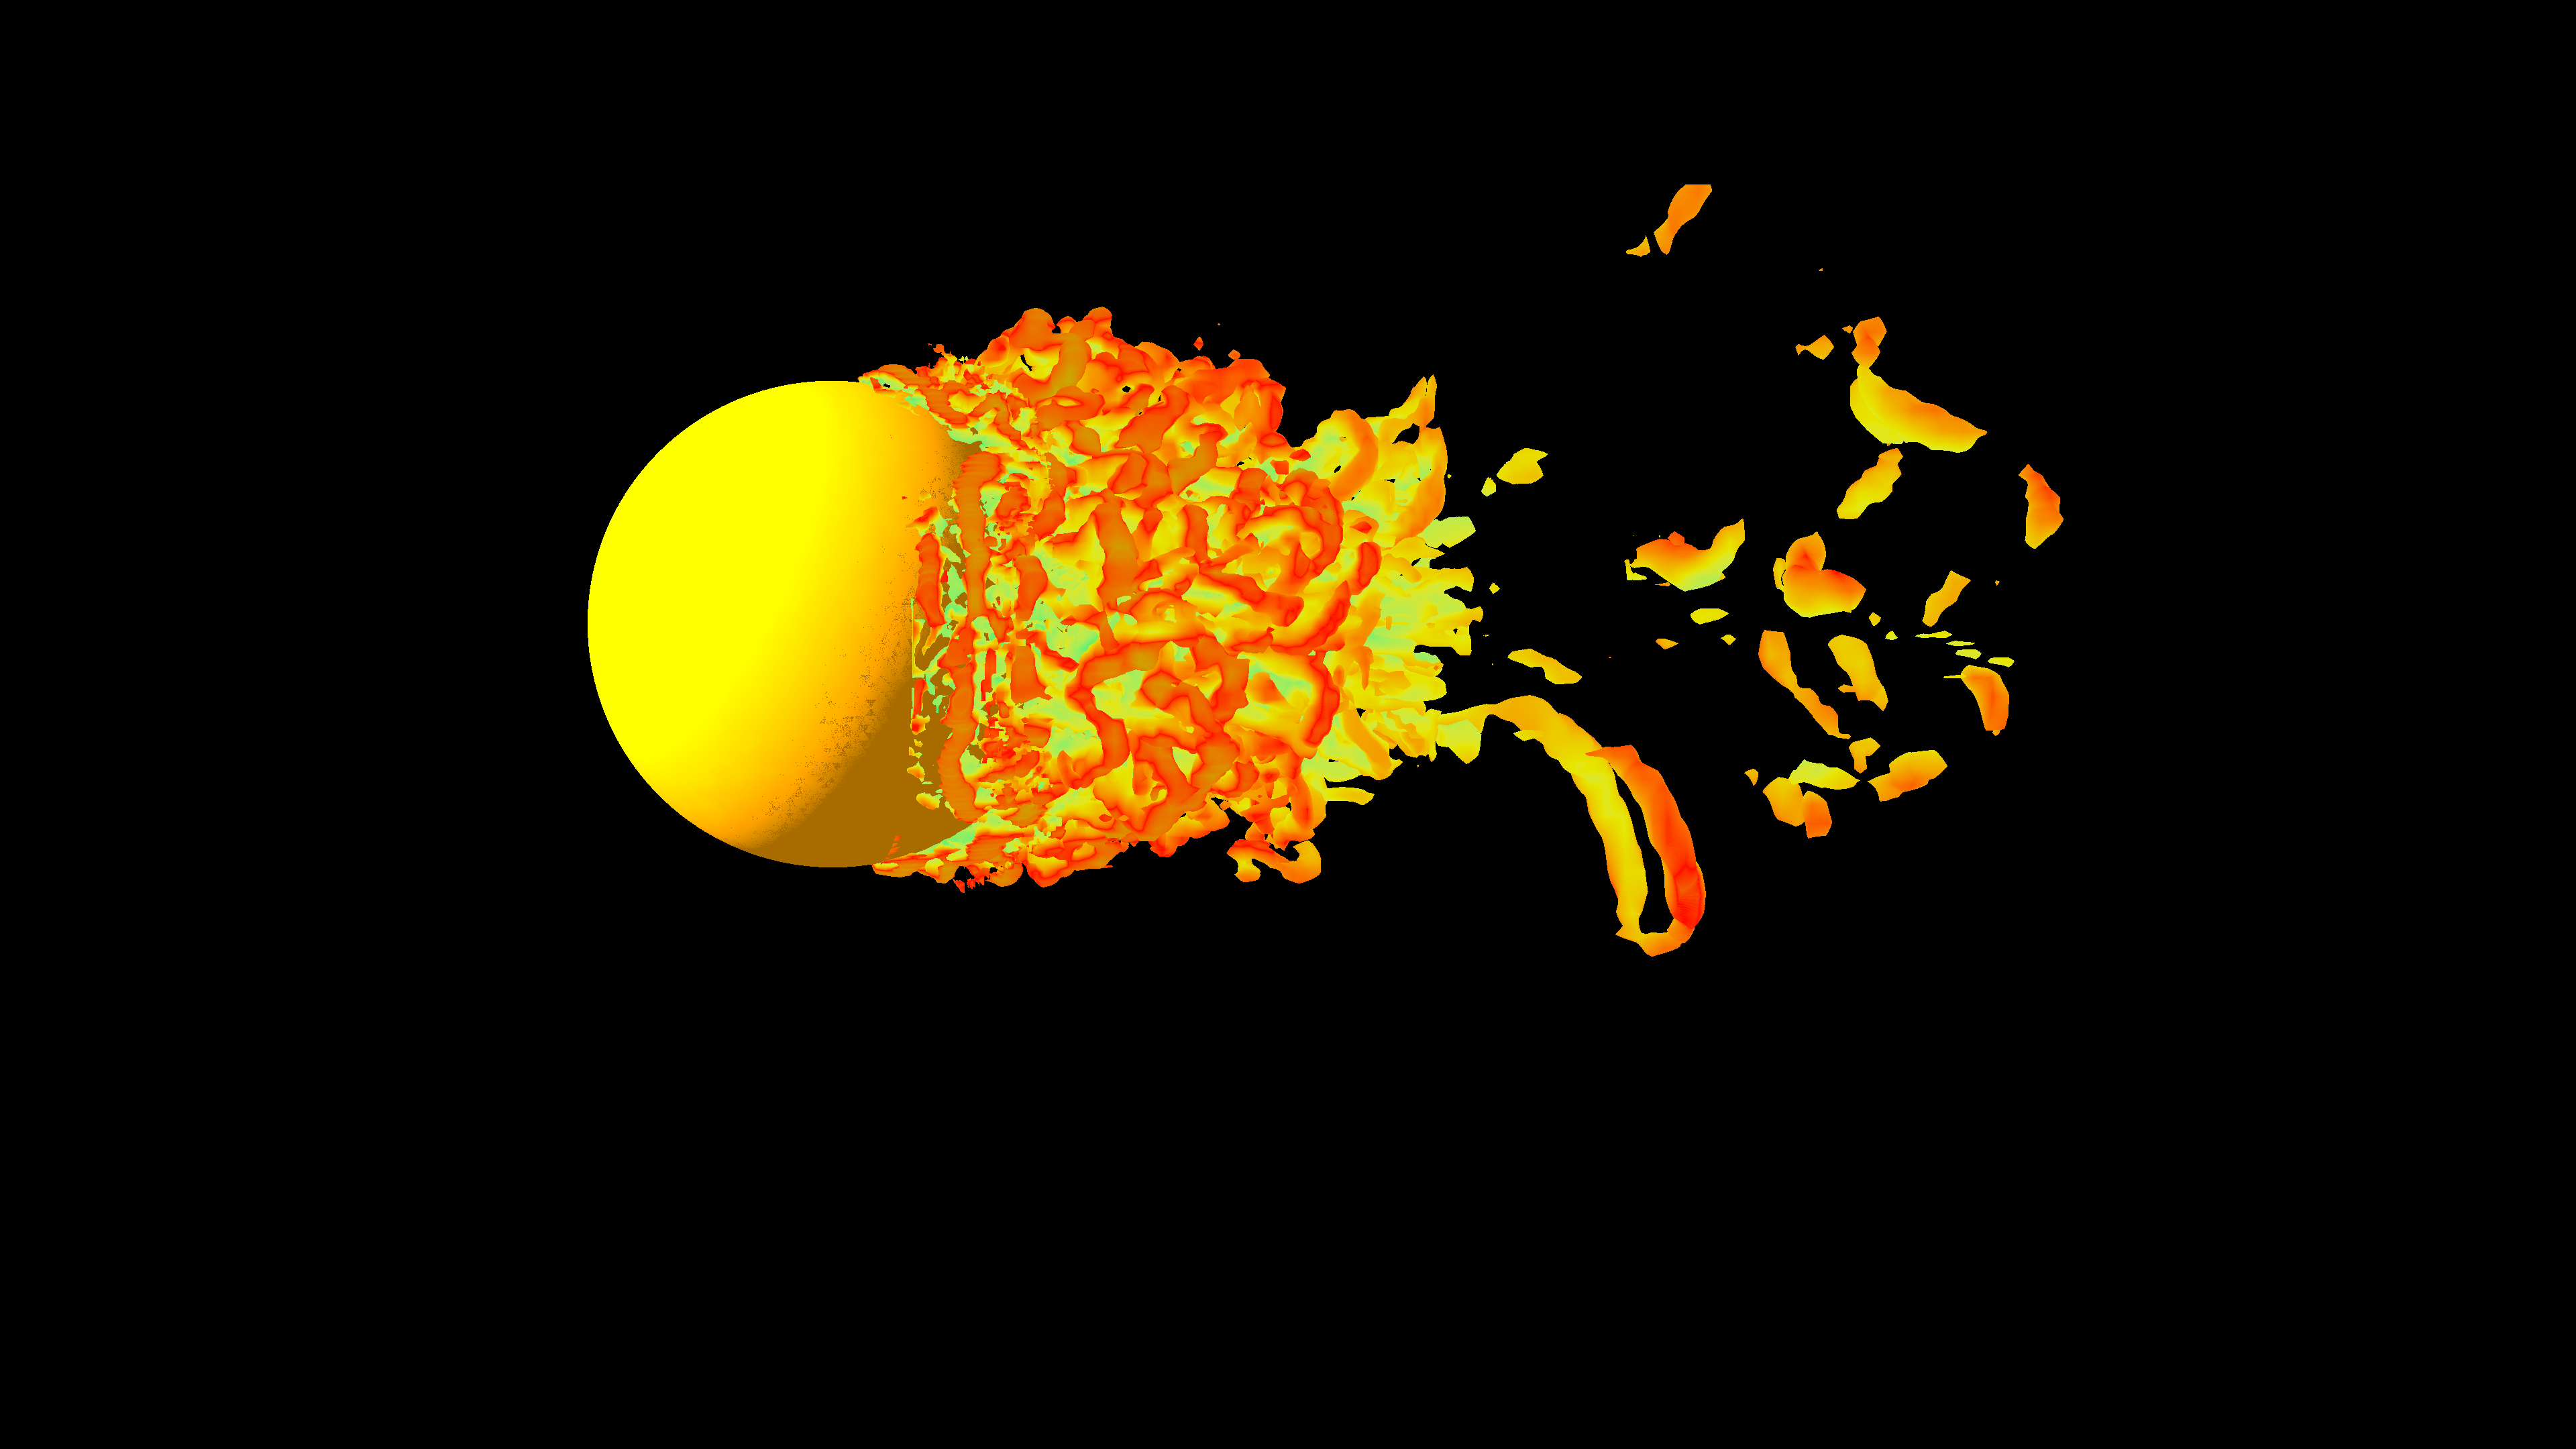
\includegraphics[width=0.45\textwidth]{./image/multi_small_4k_16_filter}
        \caption{Multi-resolution small field, 4k resolution, $ \frac{dx}{16} $ step size with object filtering (iso-value = 0.05)}\label{fig:figure5}
    \end{figure}

    \begin{figure}[H]
        \centering
        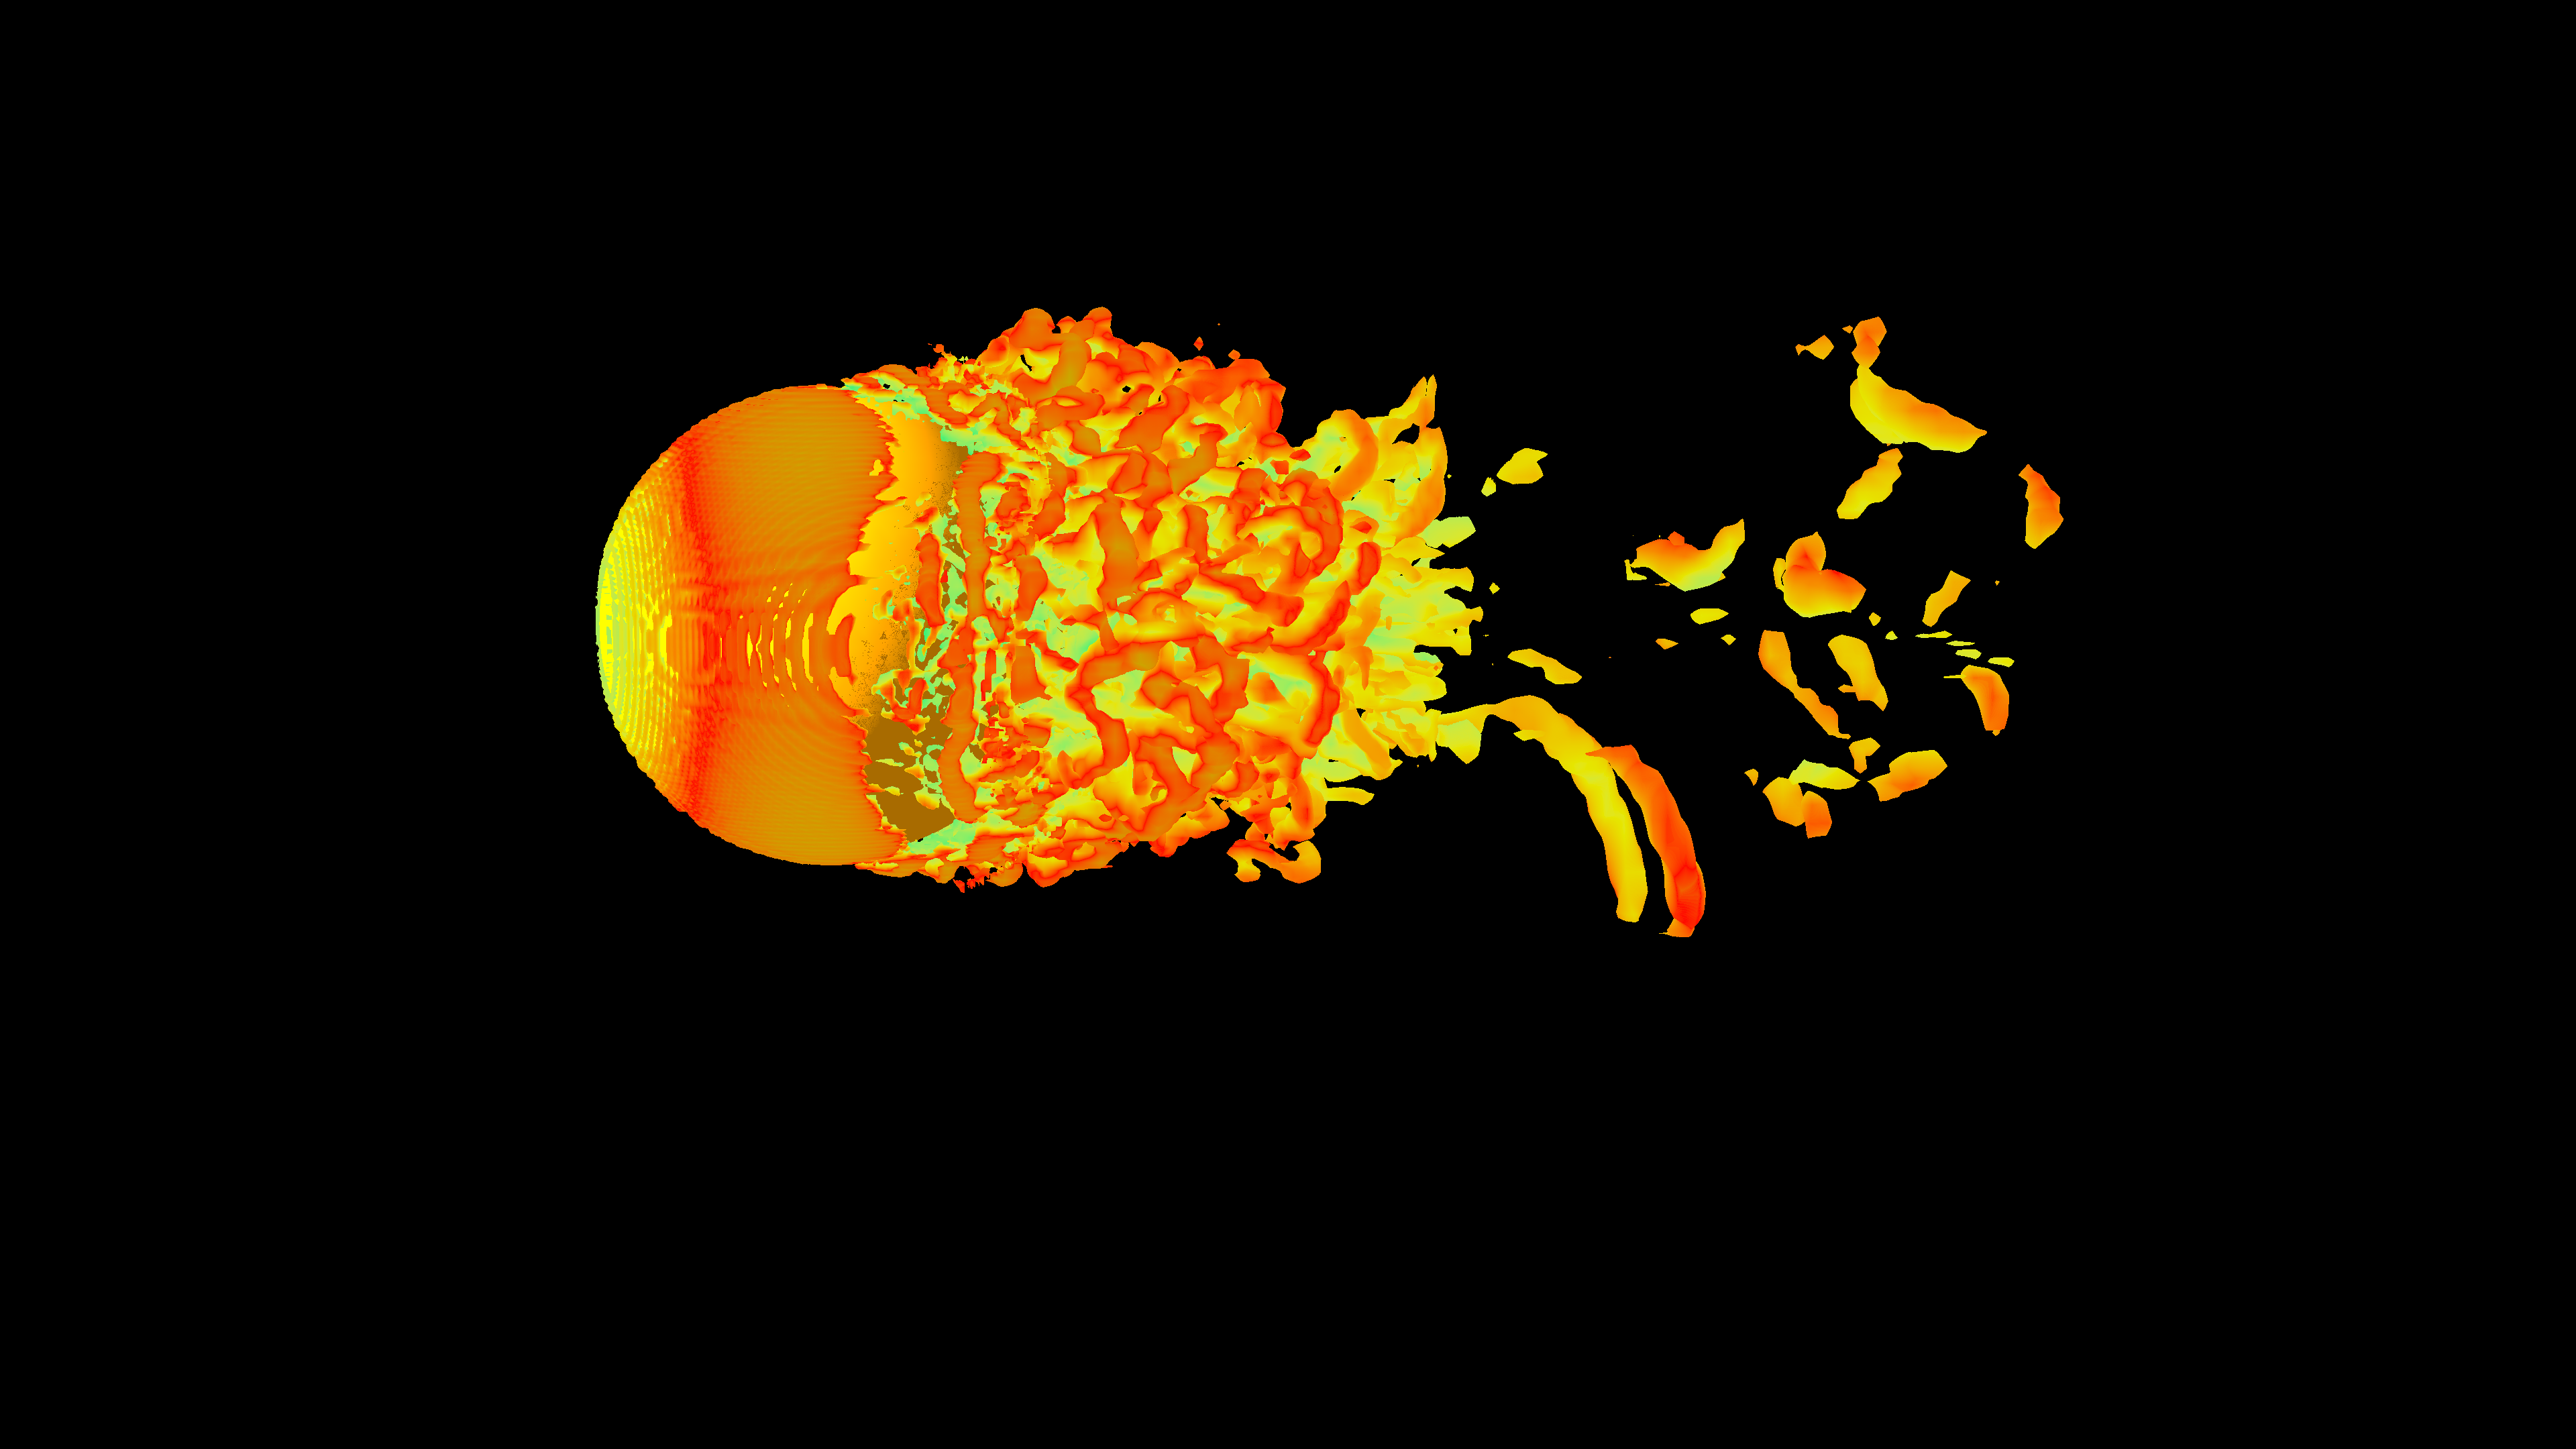
\includegraphics[width=0.45\textwidth]{./image/multi_small_4k_16_no_filter}
        \caption{Multi-resolution small field, 4k resolution, $ \frac{dx}{16} $ step size without object filtering (iso-value = 0.05)}\label{fig:figure6}
    \end{figure}

    \begin{figure}[H]
        \centering
        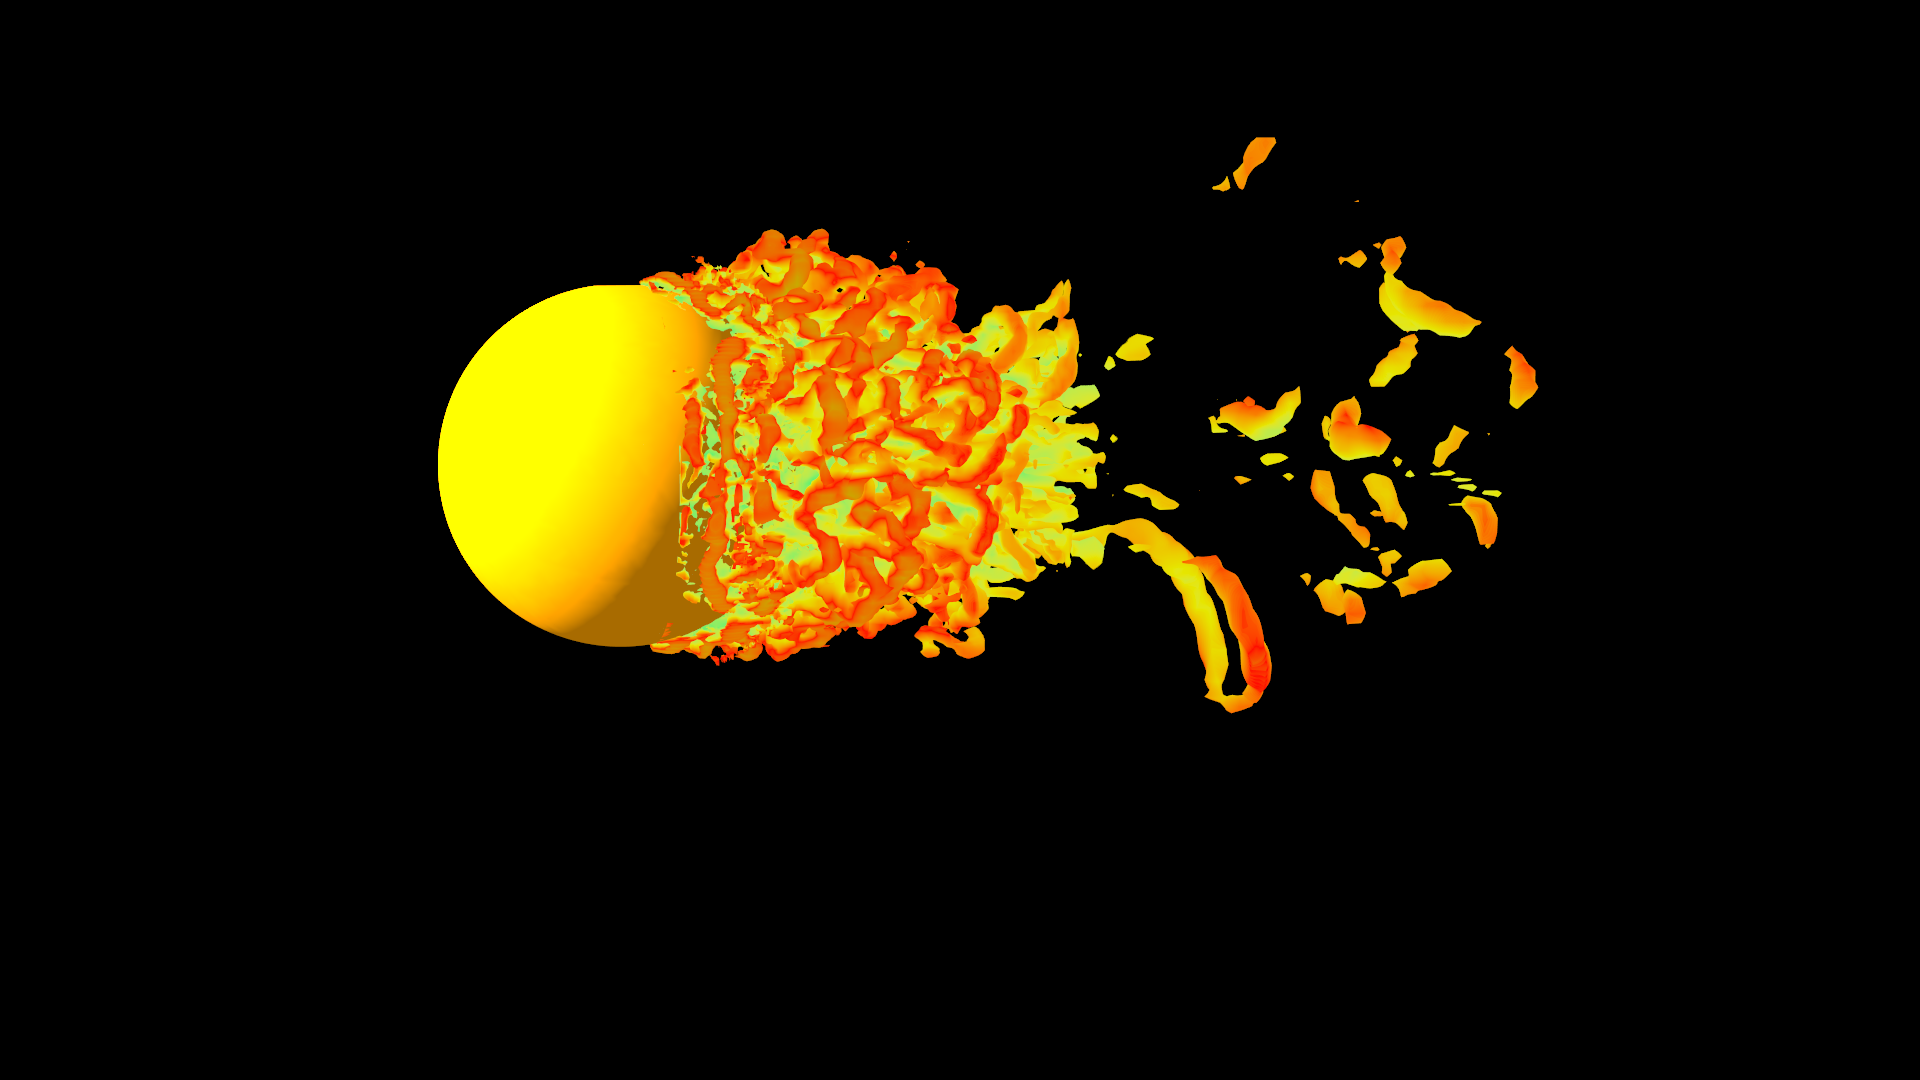
\includegraphics[width=0.45\textwidth]{./image/multi_small_1080p_8_filter_4XRES}
        \caption{Multi-resolution small field, 1080p resolution, $ \frac{dx}{8} $ step size with object filtering and 4X super resolution anti-aliasing (iso-value = 0.05)}\label{fig:figure7}
    \end{figure}

    \begin{figure}[H]
        \centering
        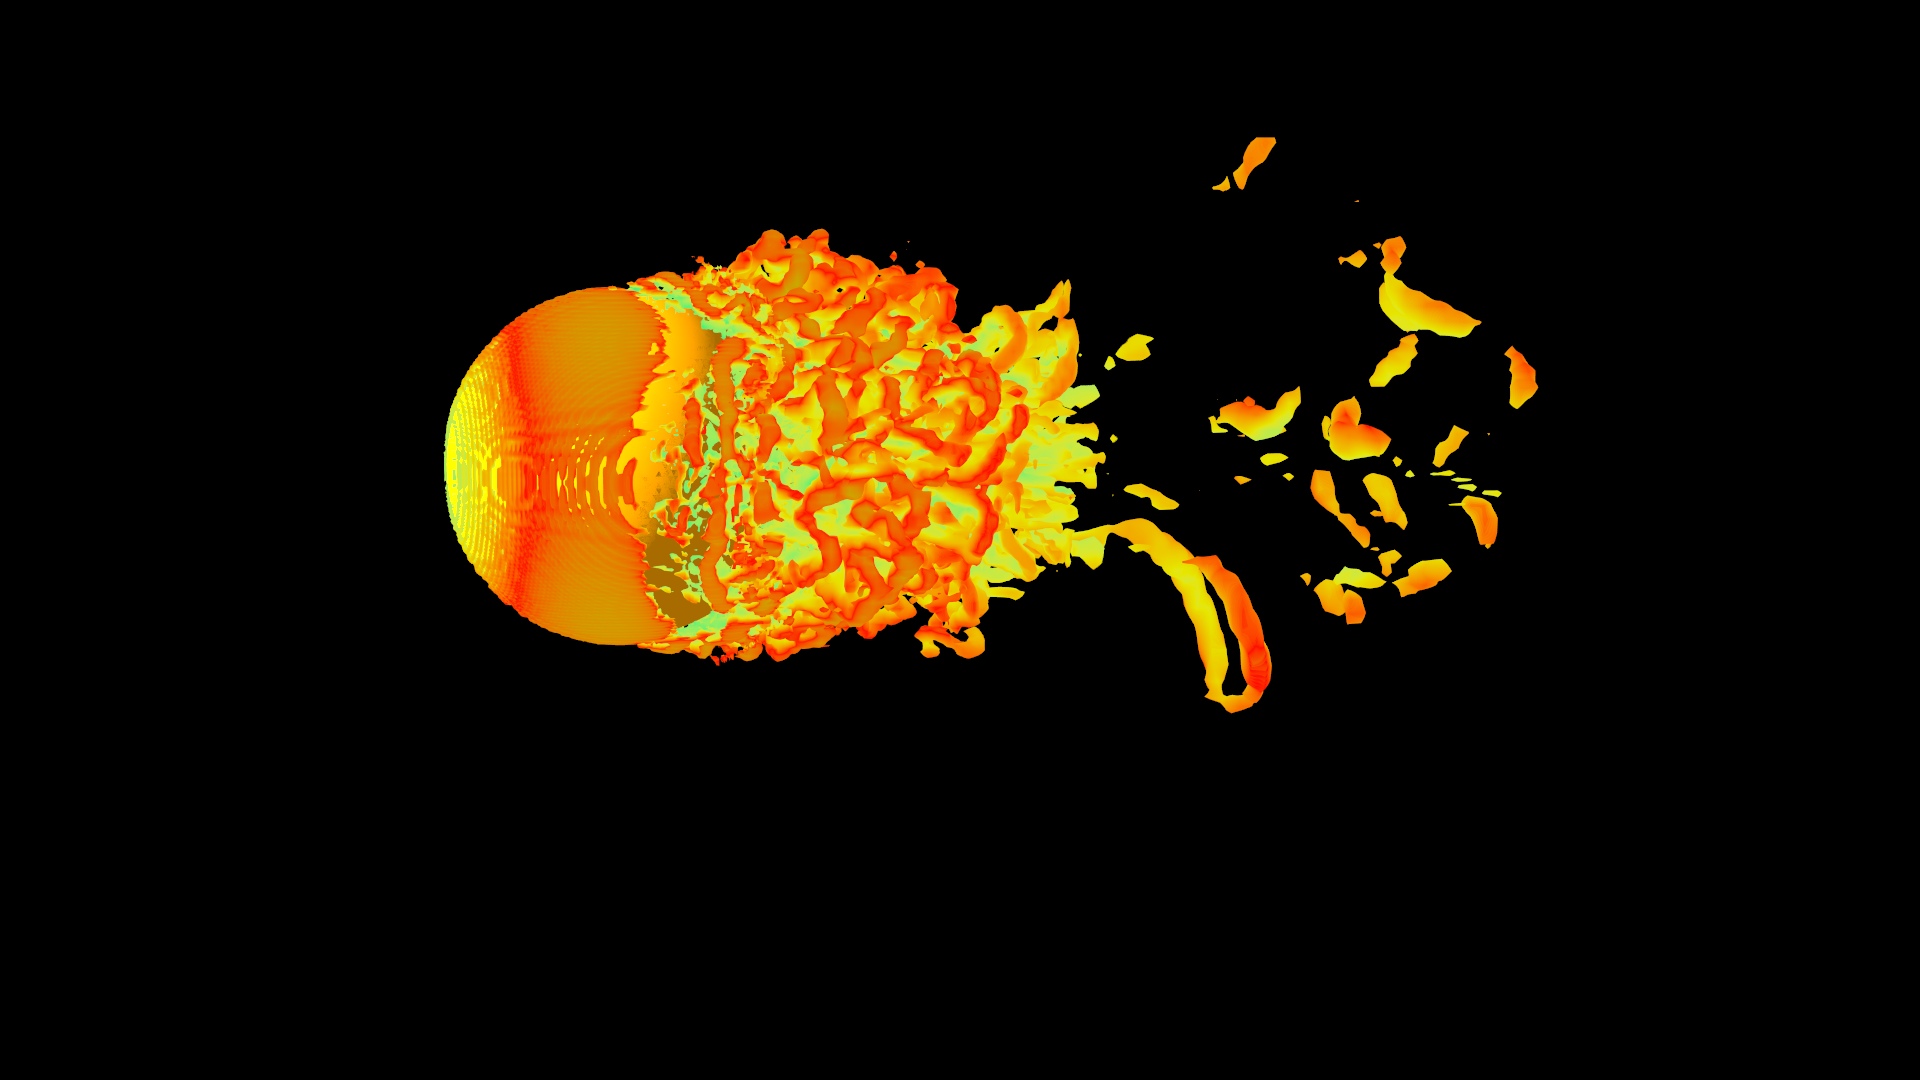
\includegraphics[width=0.45\textwidth]{./image/multi_small_1080p_8_no_filter_4XRES}
        \caption{Multi-resolution small field, 1080p resolution, $ \frac{dx}{8} $ step size without object filtering and 4X super resolution anti-aliasing (iso-value = 0.05)}\label{fig:figure8}
    \end{figure}

    \subsection{single-resolution big model}\label{subsec:single-resolution-big-model}
    \begin{figure}[H]
        \centering
        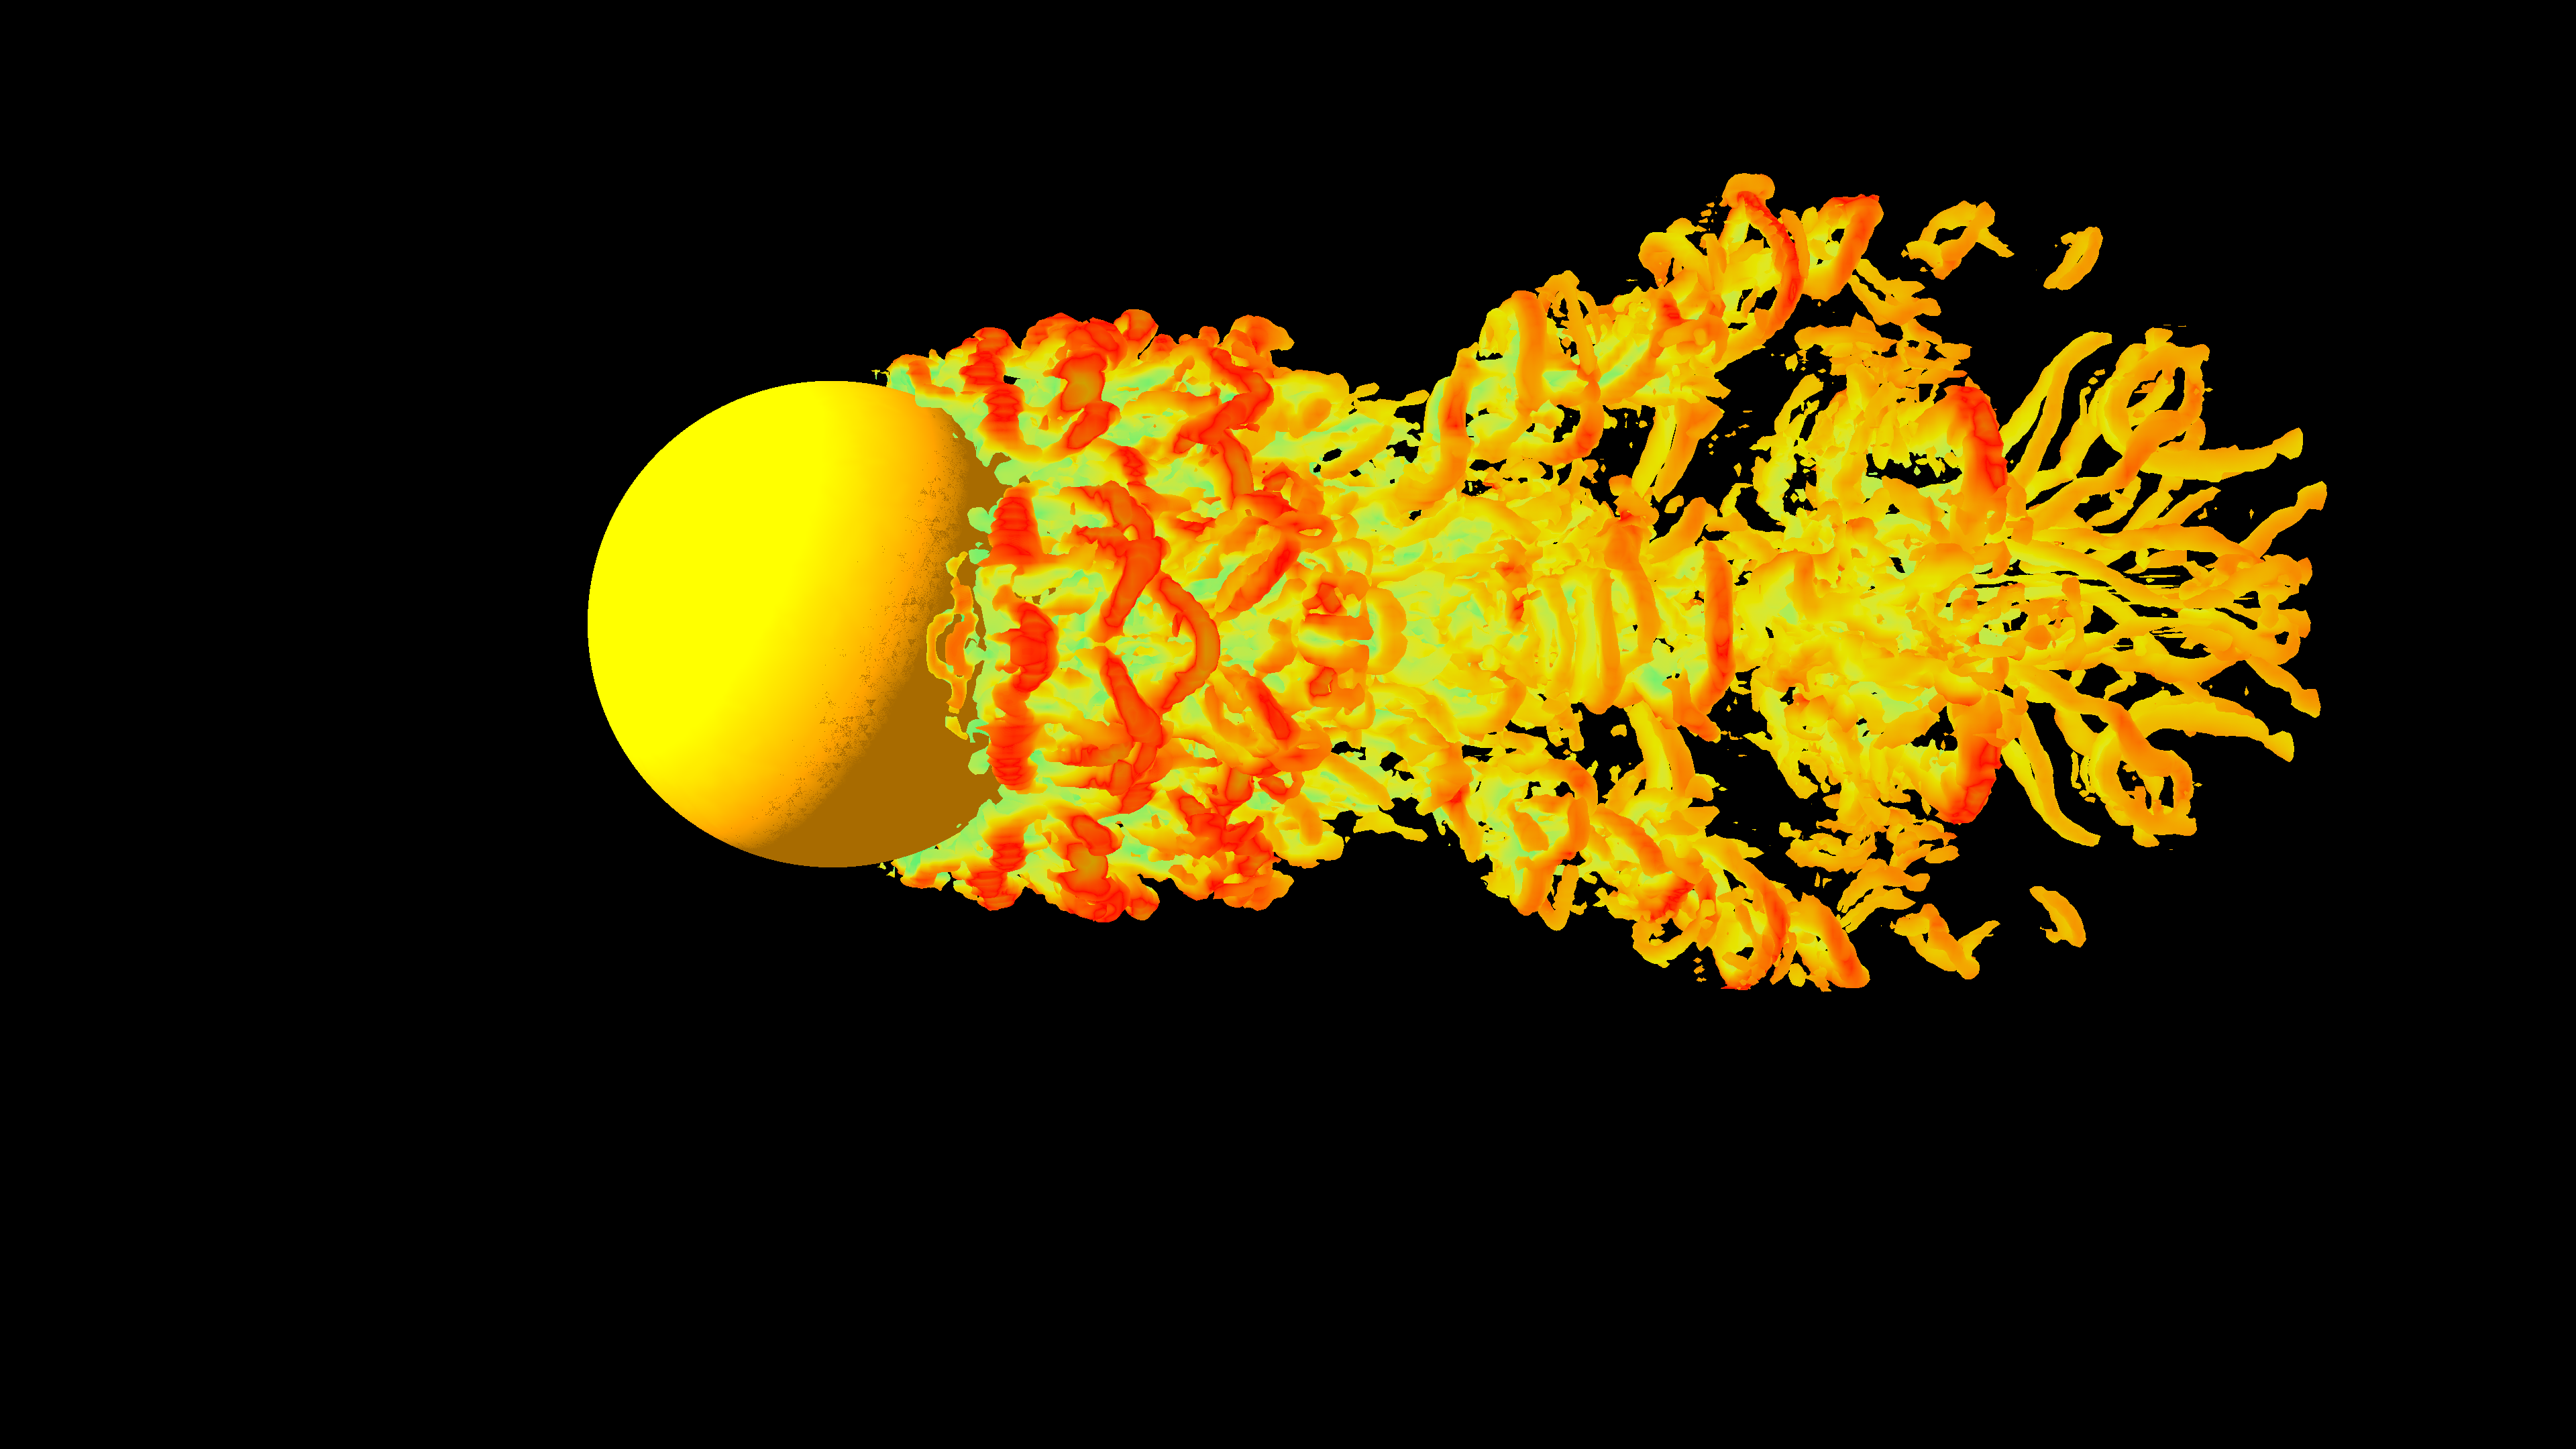
\includegraphics[width=0.45\textwidth]{./image/single_big_4k_16_filter}
        \caption{Single-resolution big field, 4k resolution, $ \frac{dx}{16} $ step size with object filtering (iso-value = 0.05)}\label{fig:figure9}
    \end{figure}

    \begin{figure}[H]
        \centering
        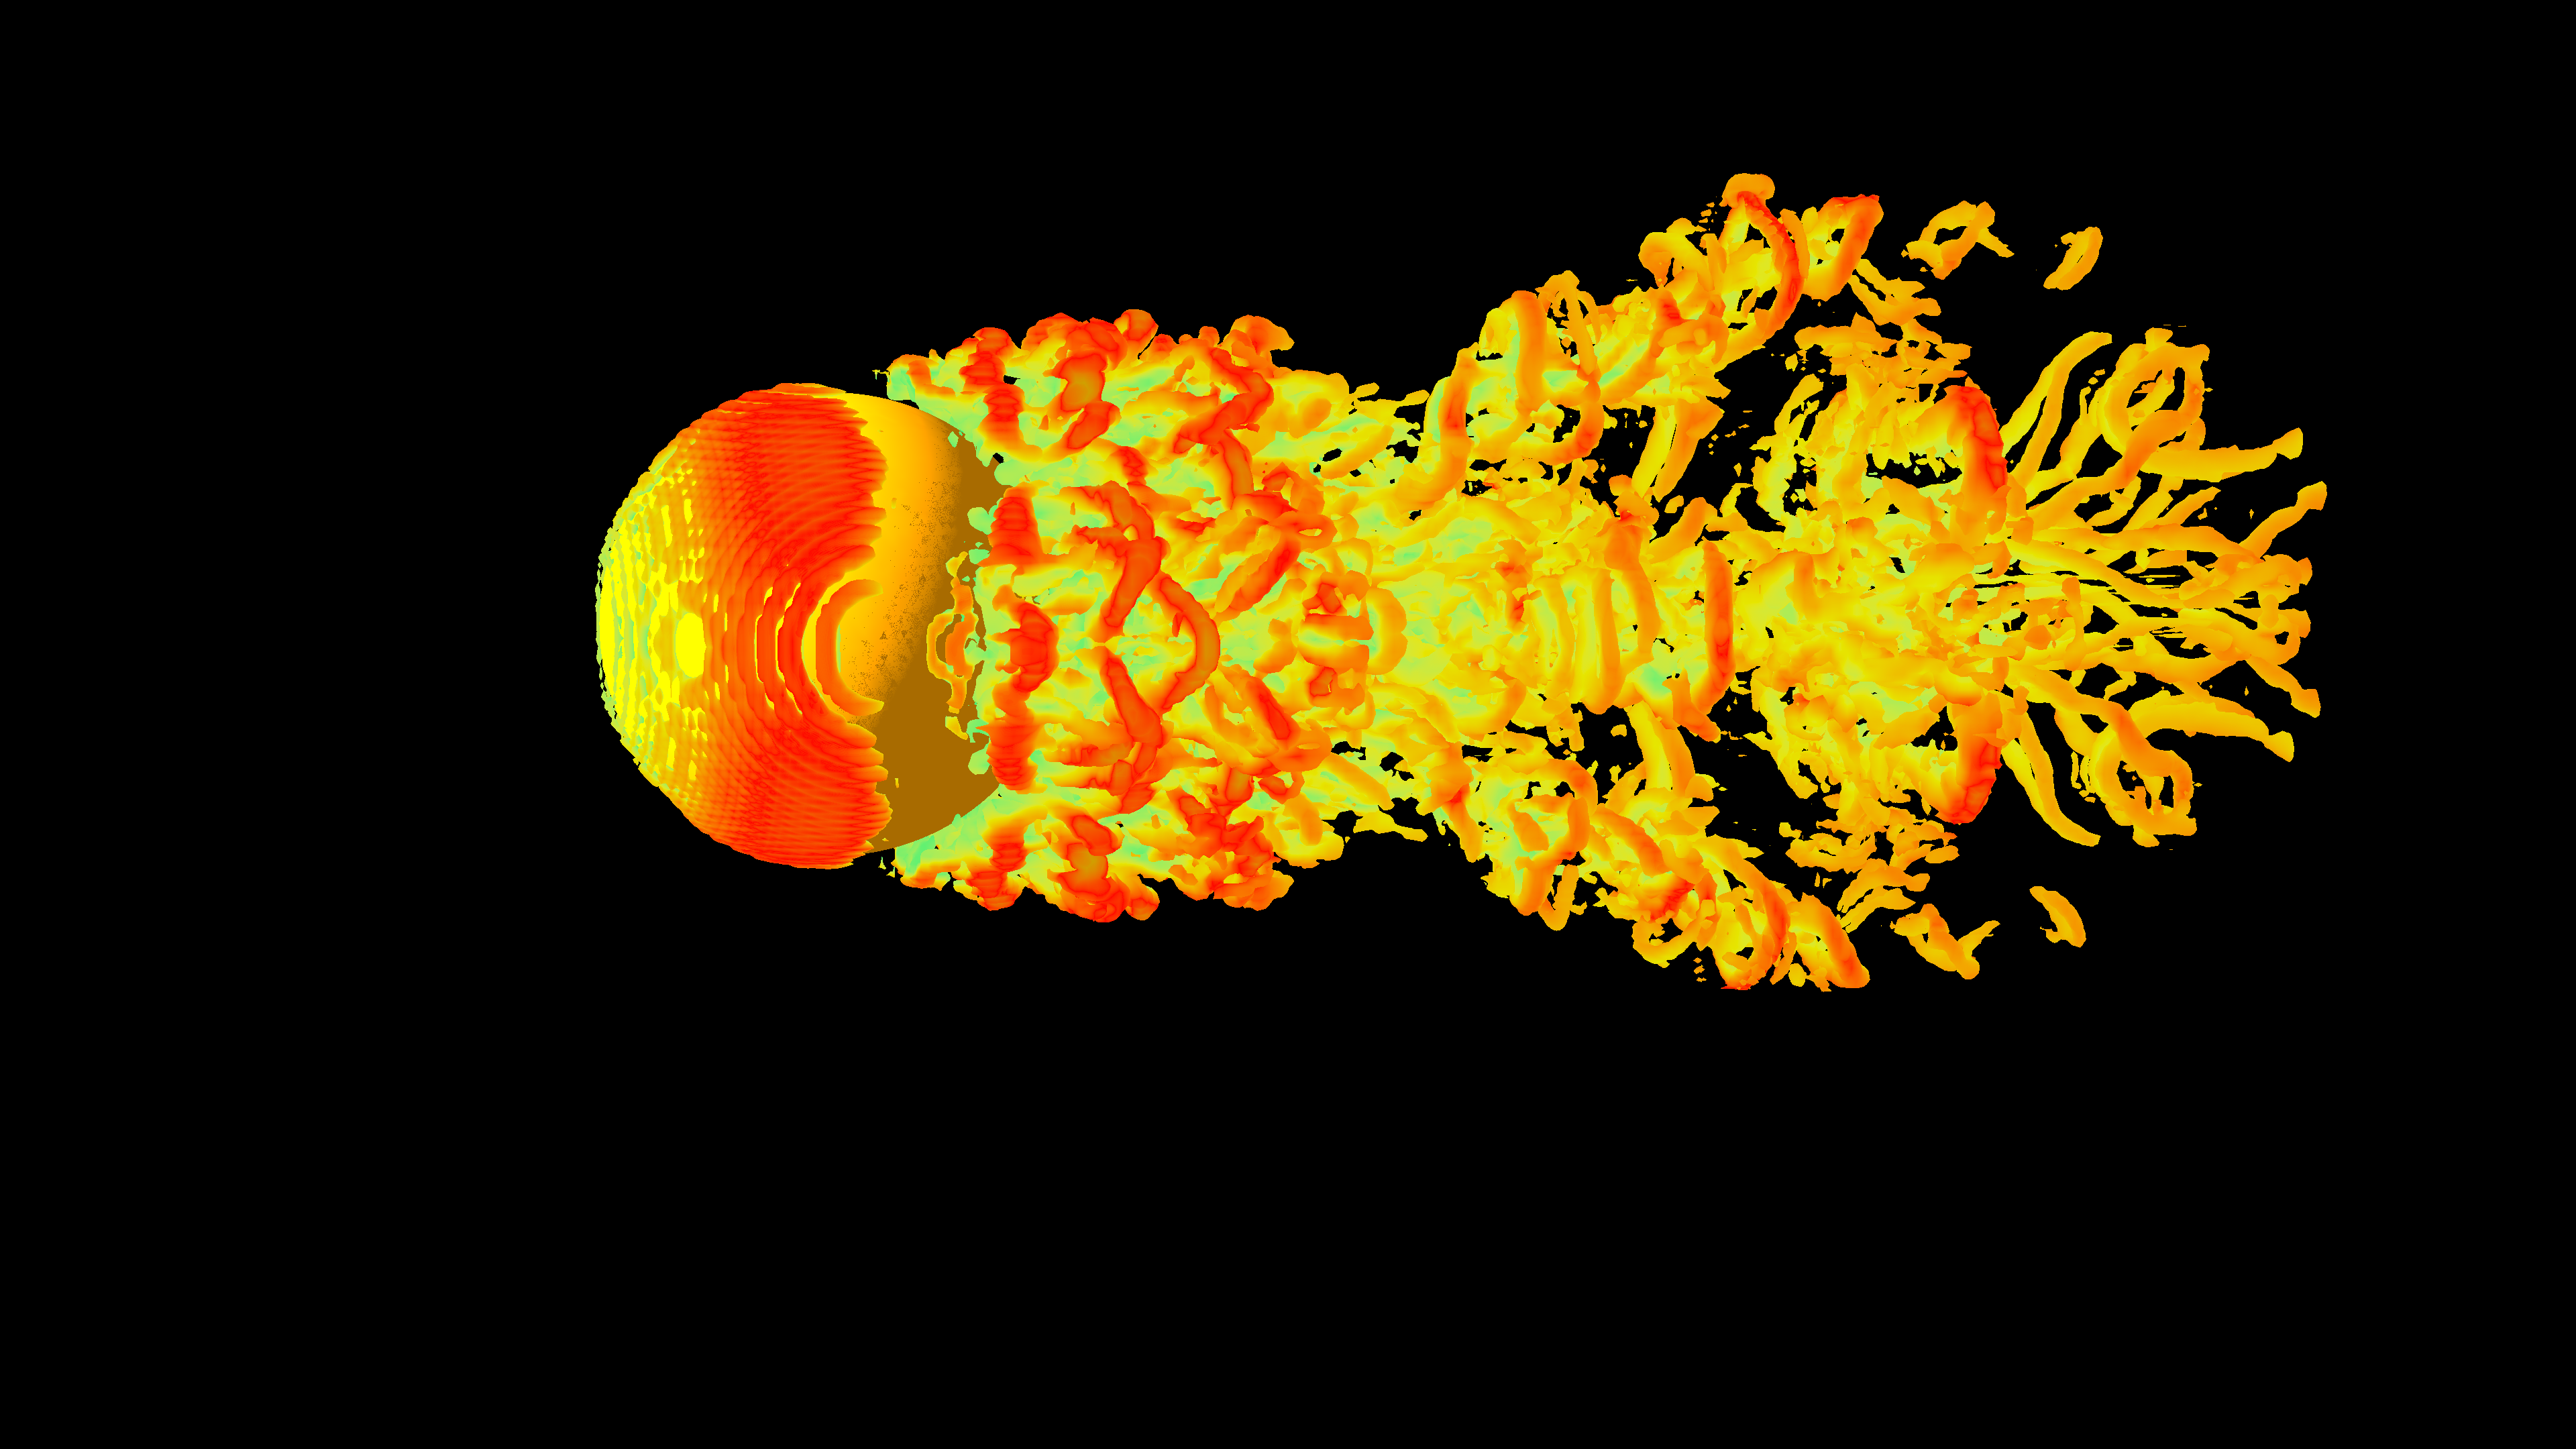
\includegraphics[width=0.45\textwidth]{./image/single_big_4k_16_no_filter}
        \caption{Single-resolution big field, 4k resolution, $ \frac{dx}{16} $ step size without object filtering (iso-value = 0.05)}\label{fig:figure10}
    \end{figure}

    \begin{figure}[H]
        \centering
        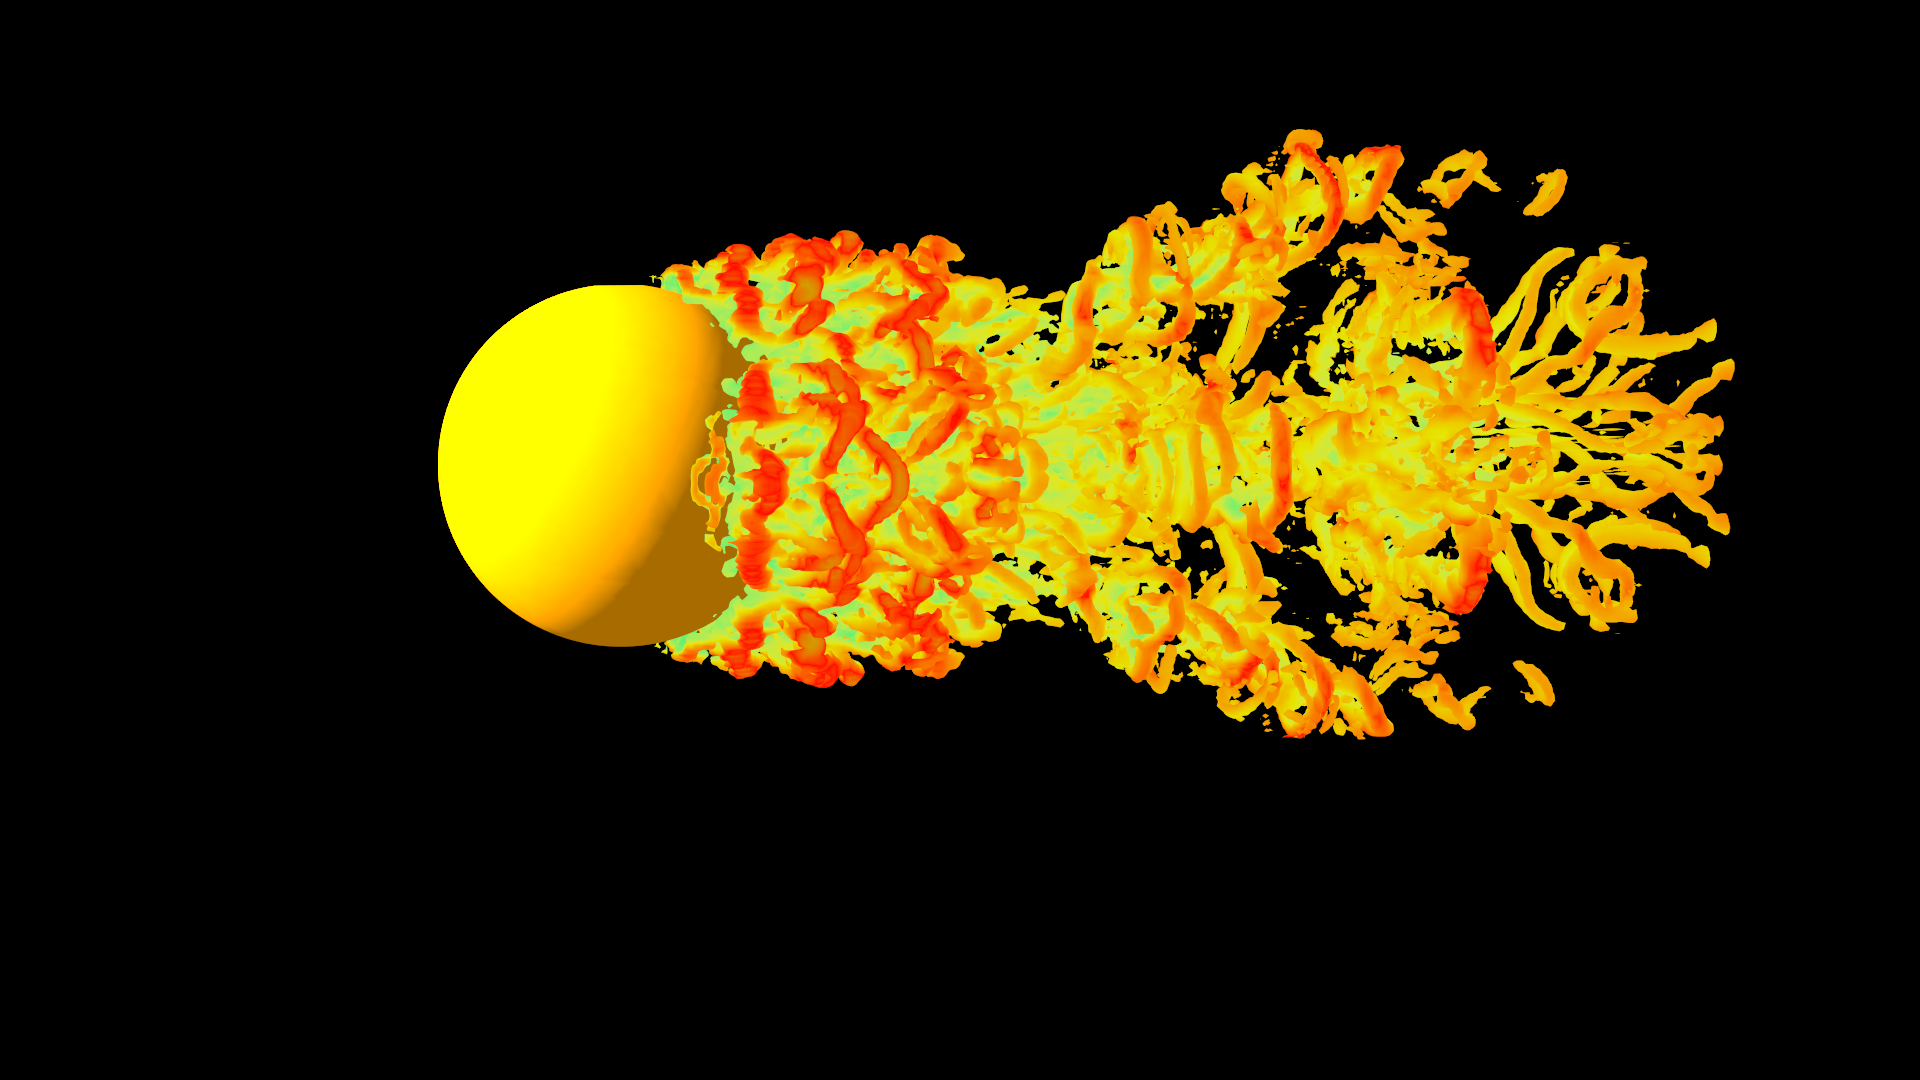
\includegraphics[width=0.45\textwidth]{./image/single_big_1080p_8_filter_4XRES}
        \caption{Single-resolution big field, 1080p resolution, $ \frac{dx}{8} $ step size with object filtering and 4X super resolution anti-aliasing (iso-value = 0.05)}\label{fig:figure11}
    \end{figure}

    \begin{figure}[H]
        \centering
        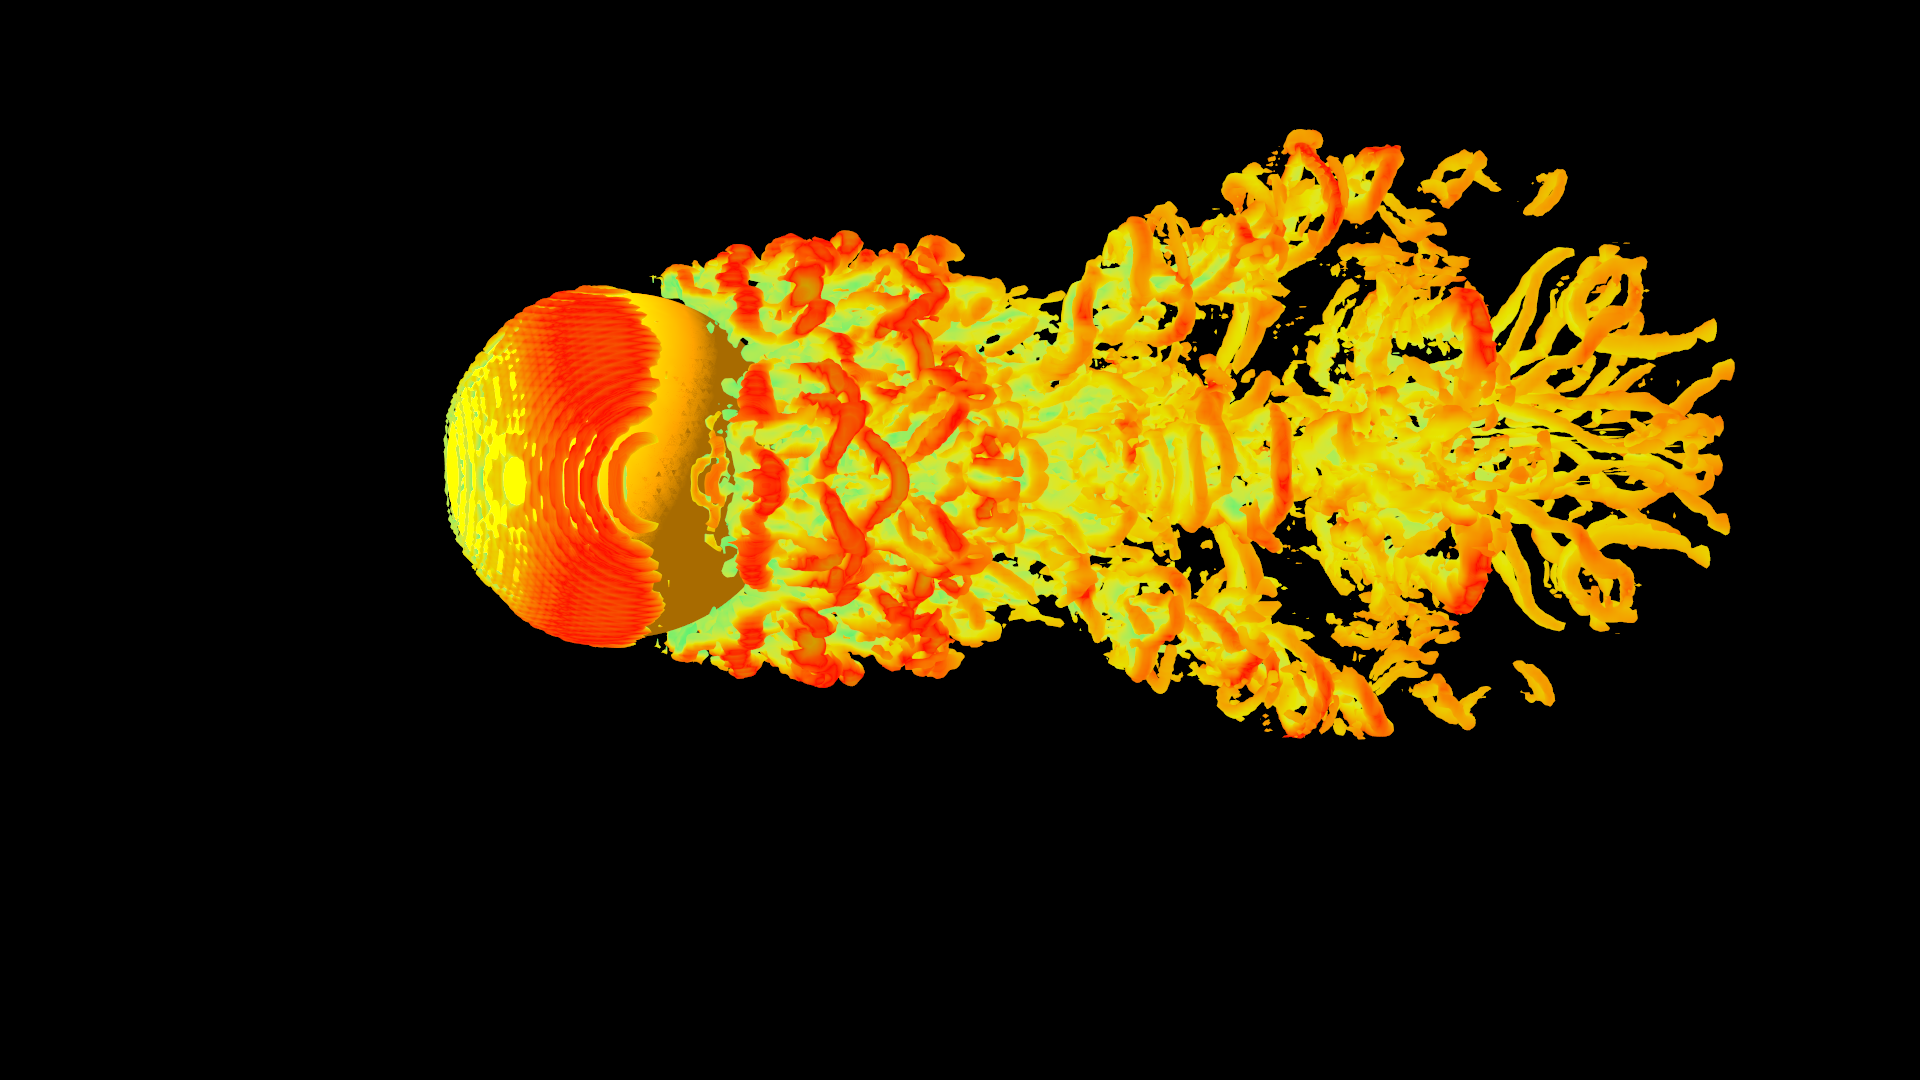
\includegraphics[width=0.45\textwidth]{./image/single_big_1080p_8_no_filter_4XRES}
        \caption{Single-resolution big field, 1080p resolution, $ \frac{dx}{8} $ step size without object filtering and 4X super resolution anti-aliasing (iso-value = 0.05)}\label{fig:figure12}
    \end{figure}

    \subsection{single-resolution small model}\label{subsec:single-resolution-small-model}
    \begin{figure}[H]
        \centering
        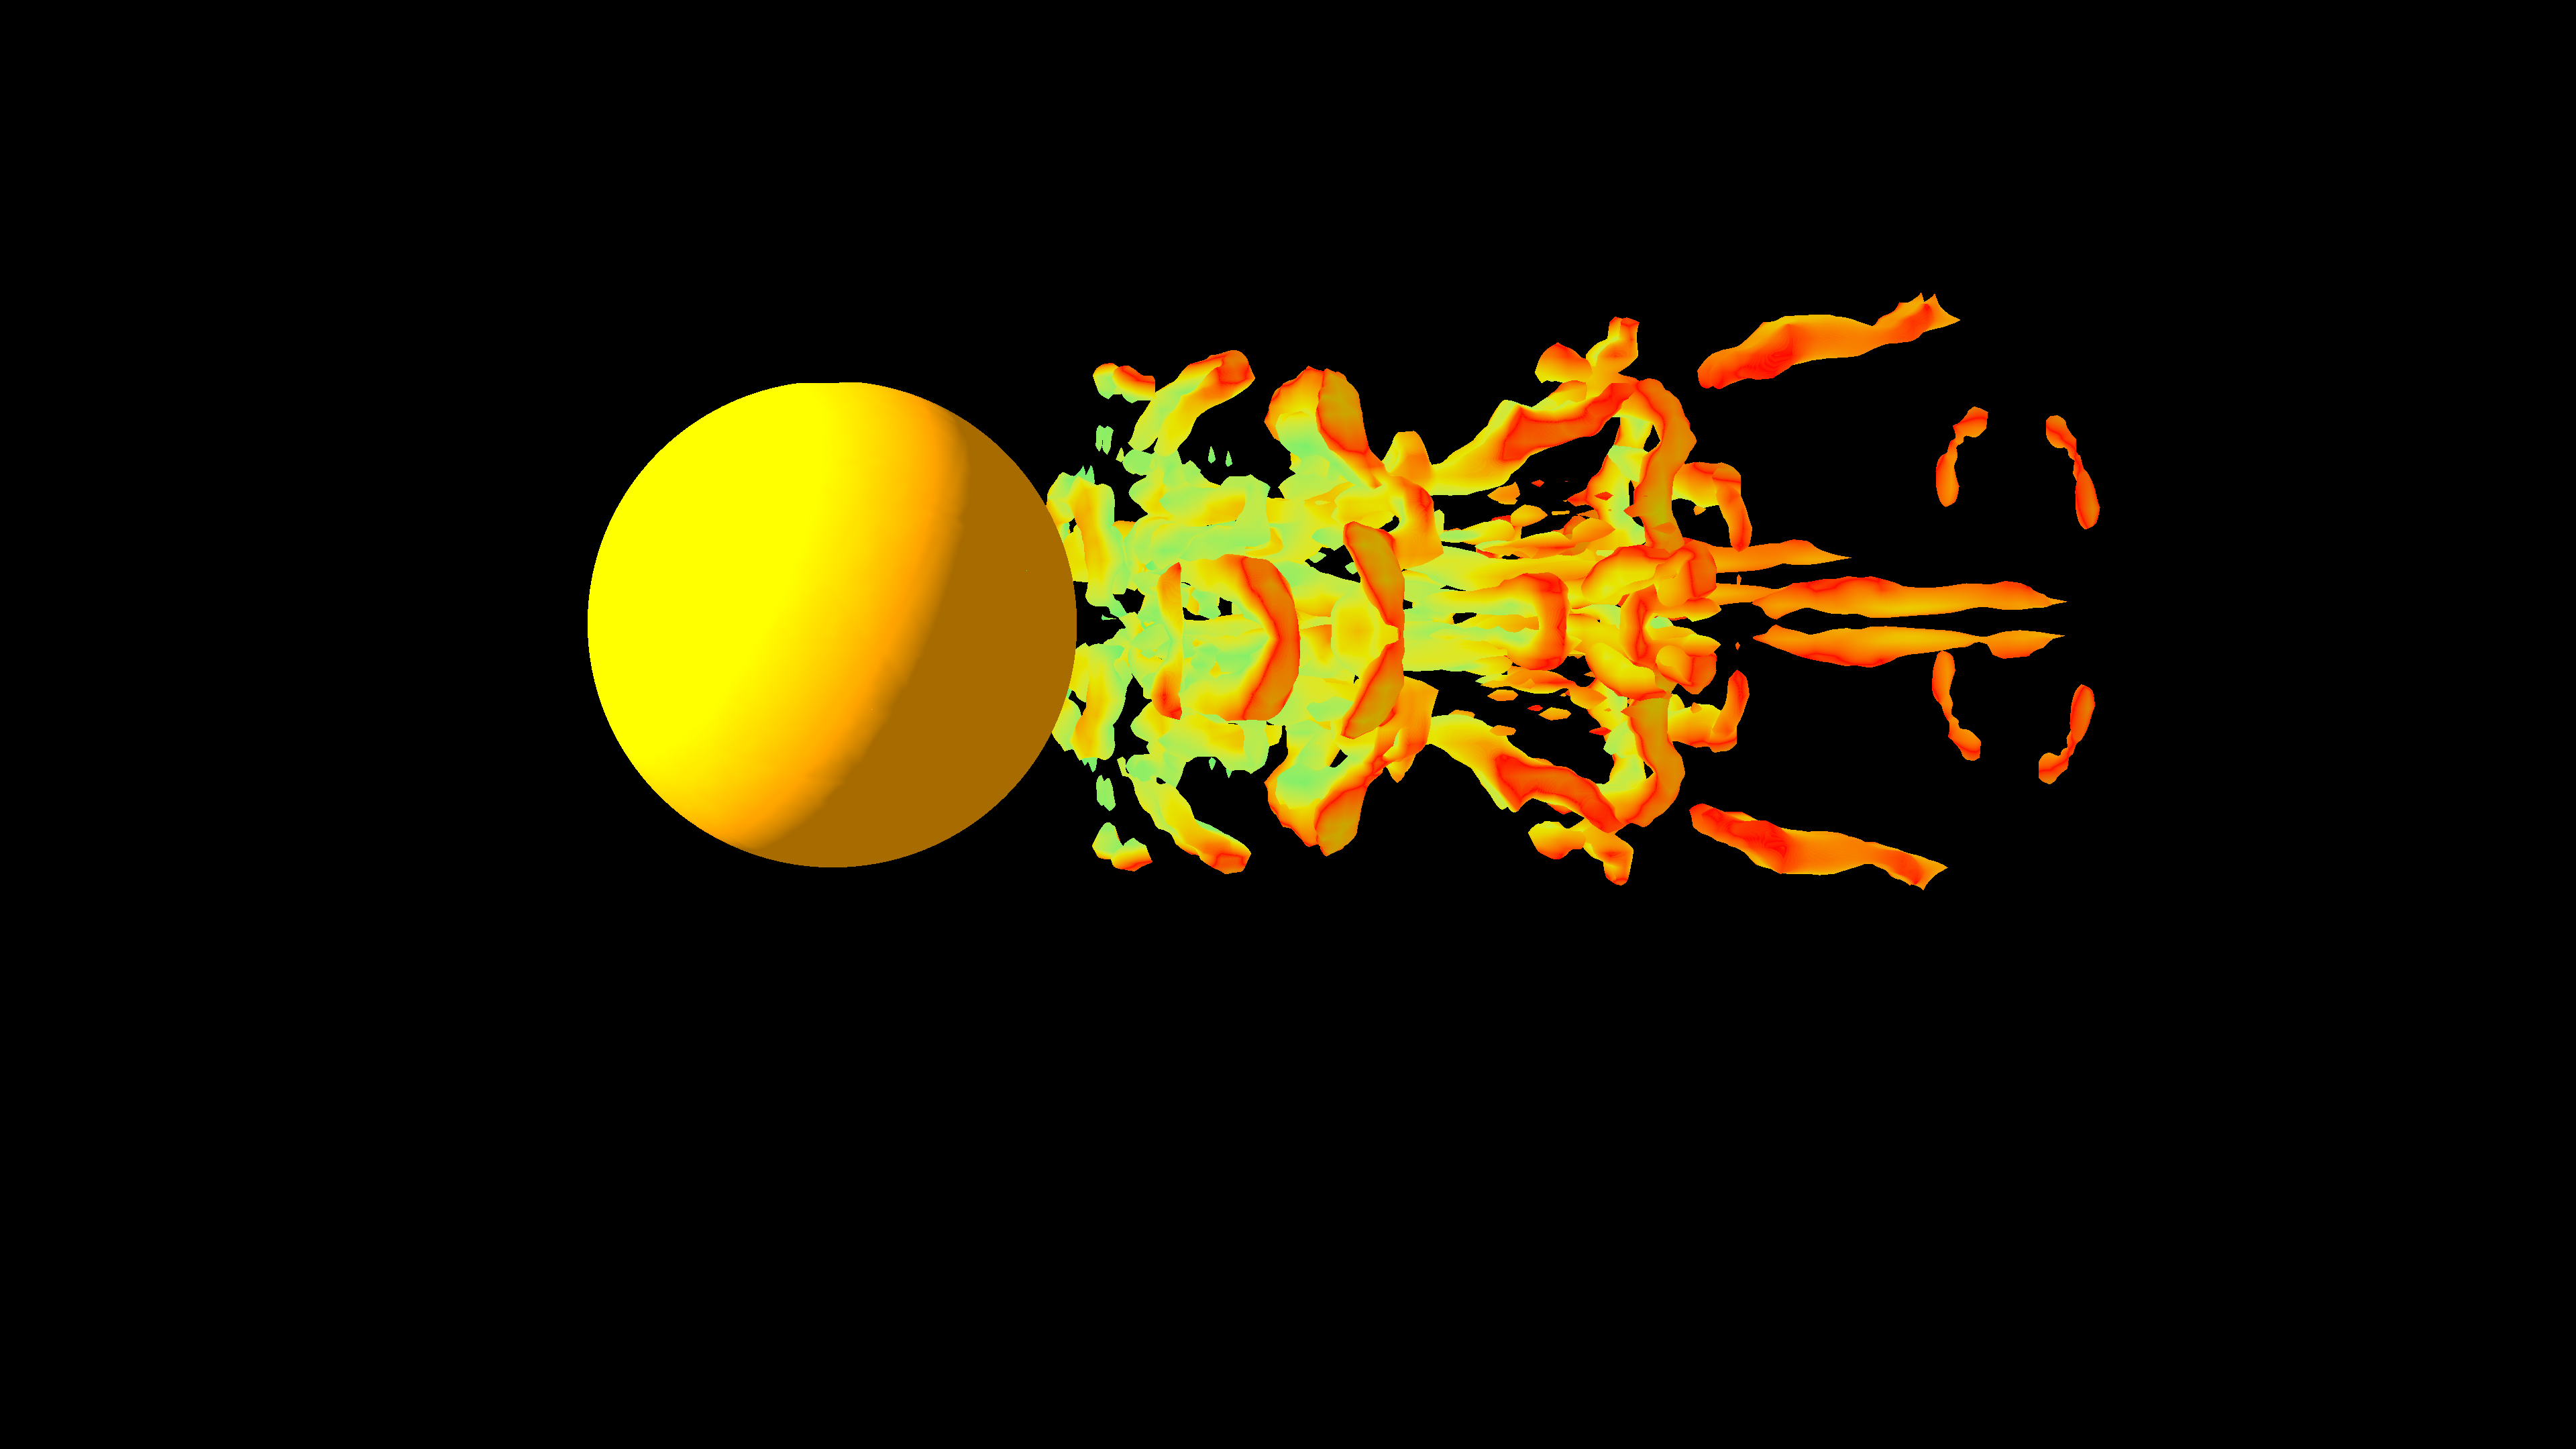
\includegraphics[width=0.45\textwidth]{./image/single_small_4k_16_filter}
        \caption{Single-resolution small field, 4k resolution, $ \frac{dx}{16} $ step size with object filtering (iso-value = 0.05)}\label{fig:figure13}
    \end{figure}

    \begin{figure}[H]
        \centering
        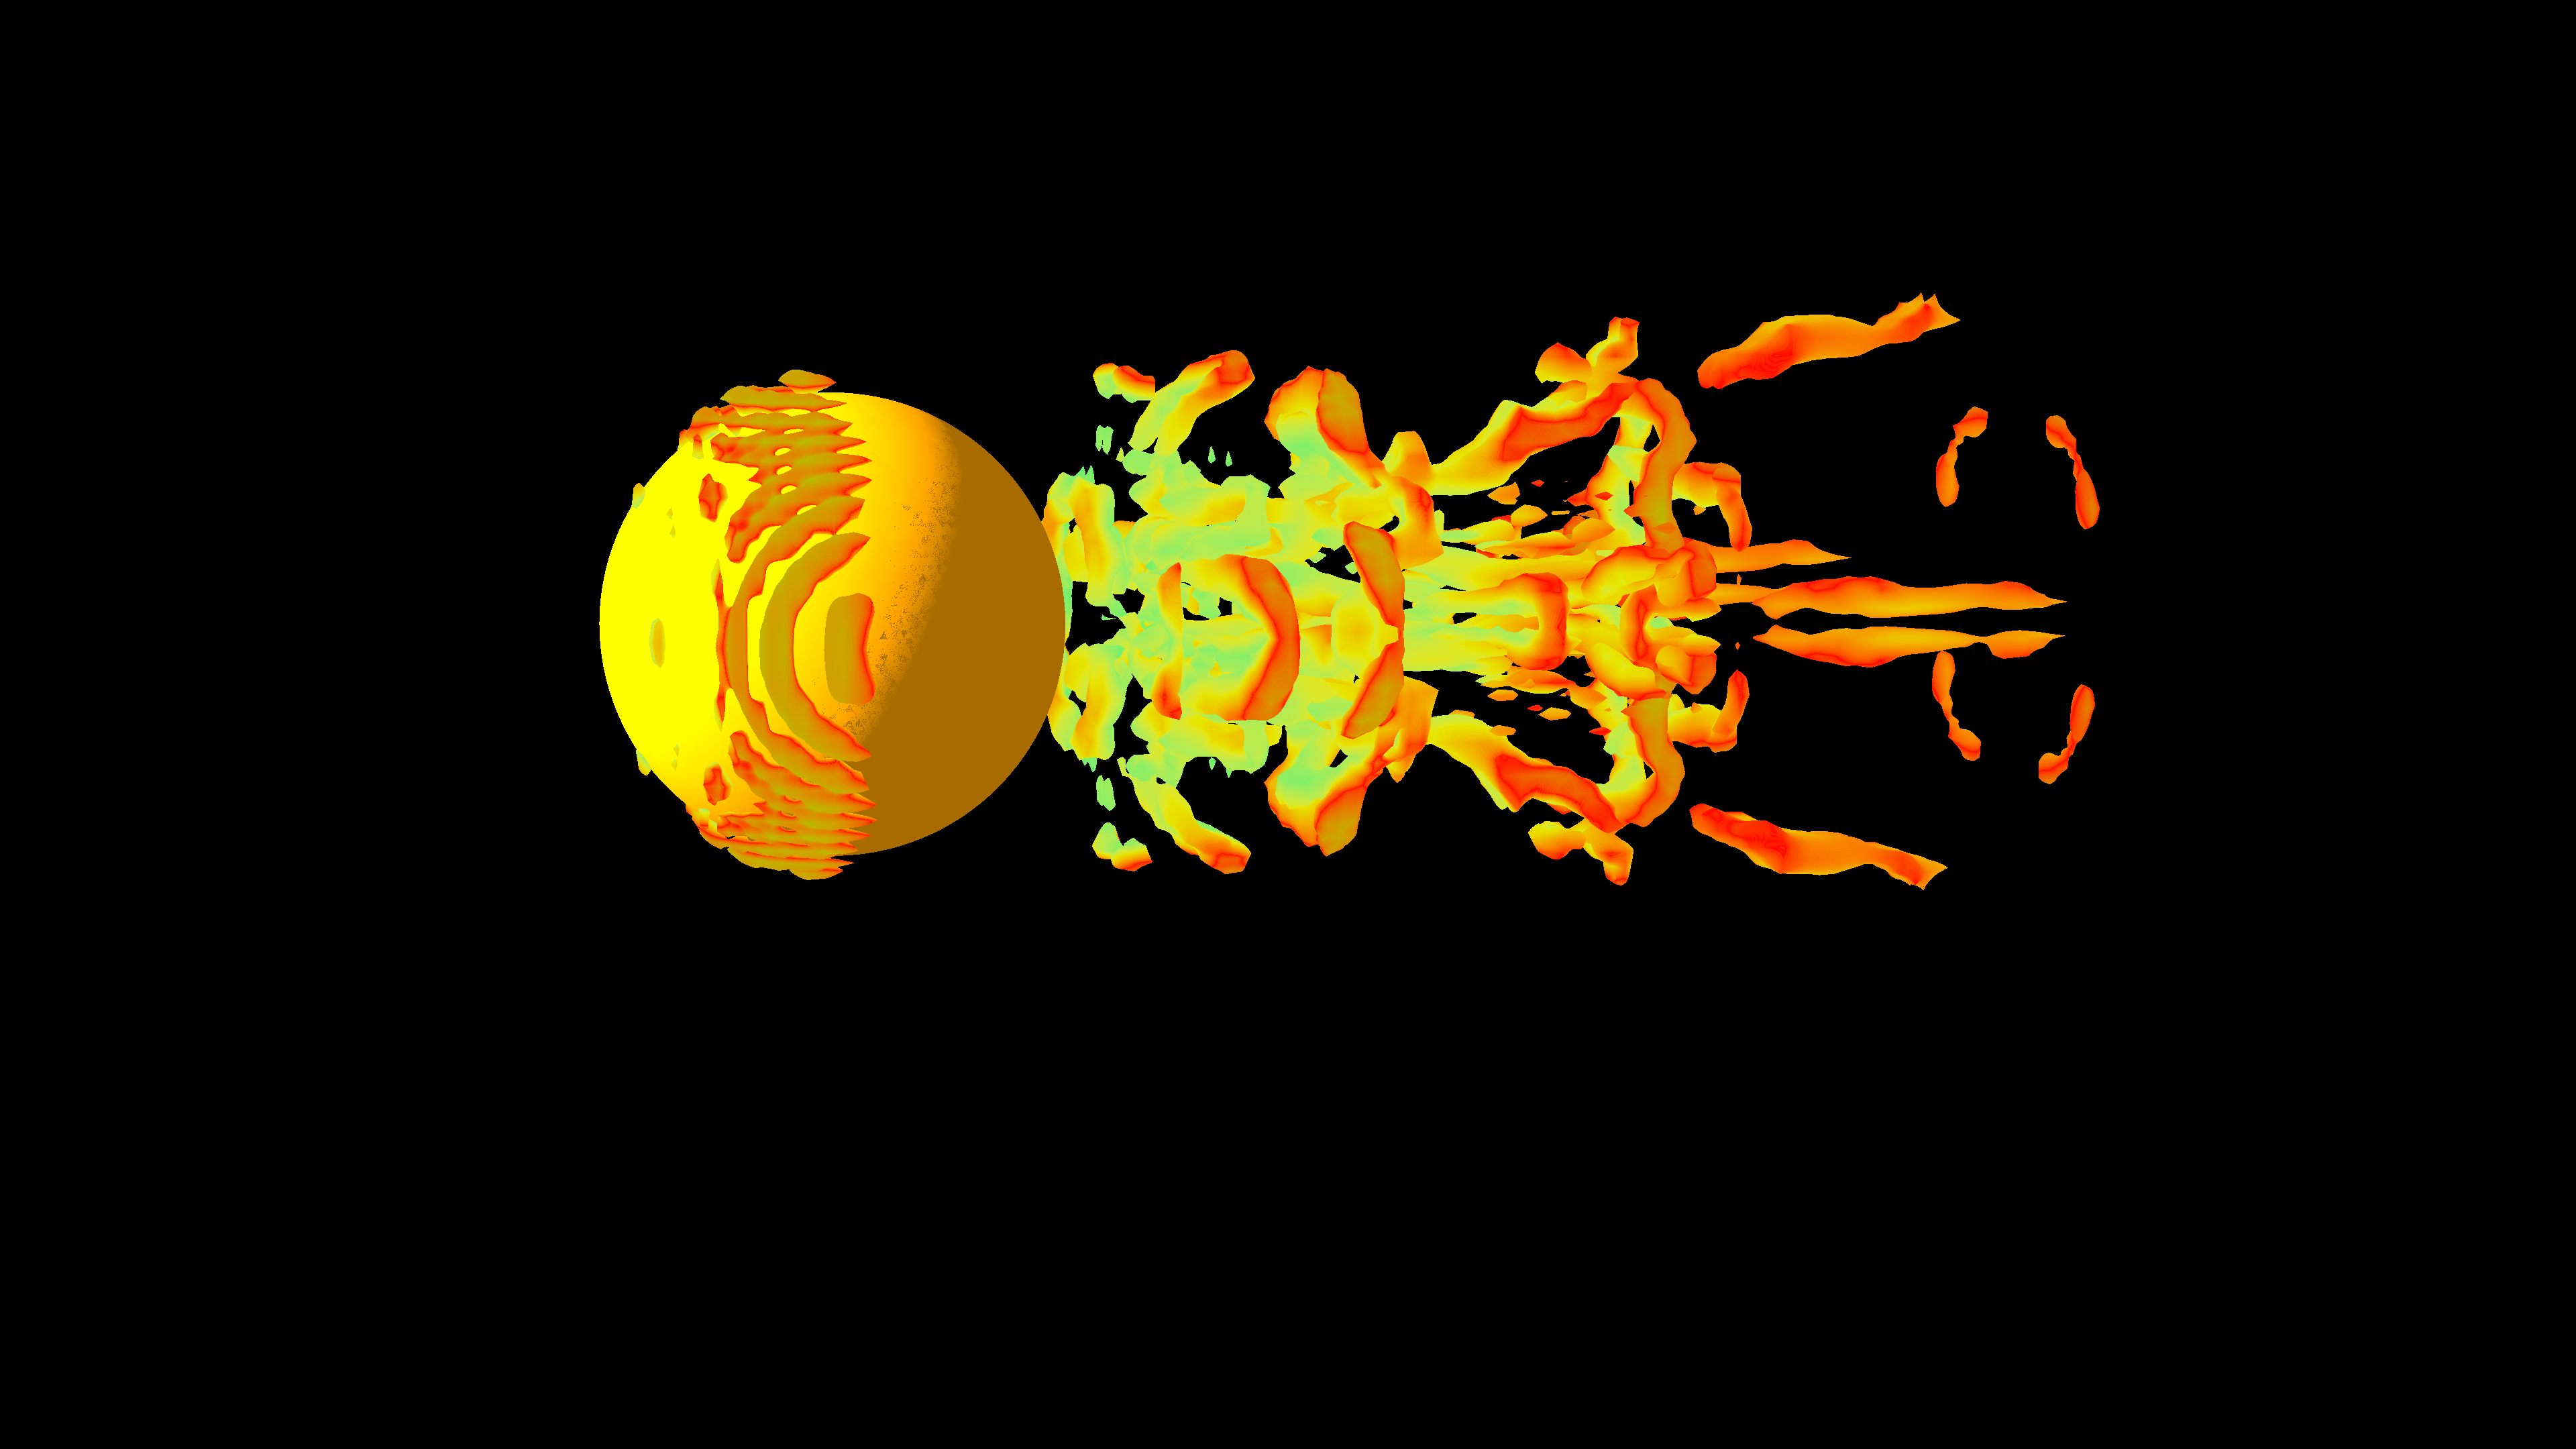
\includegraphics[width=0.45\textwidth]{./image/single_small_4k_16_no_filter}
        \caption{Single-resolution small field, 4k resolution, $ \frac{dx}{16} $ step size without object filtering (iso-value = 0.05)}\label{fig:figure14}
    \end{figure}

    \begin{figure}[H]
        \centering
        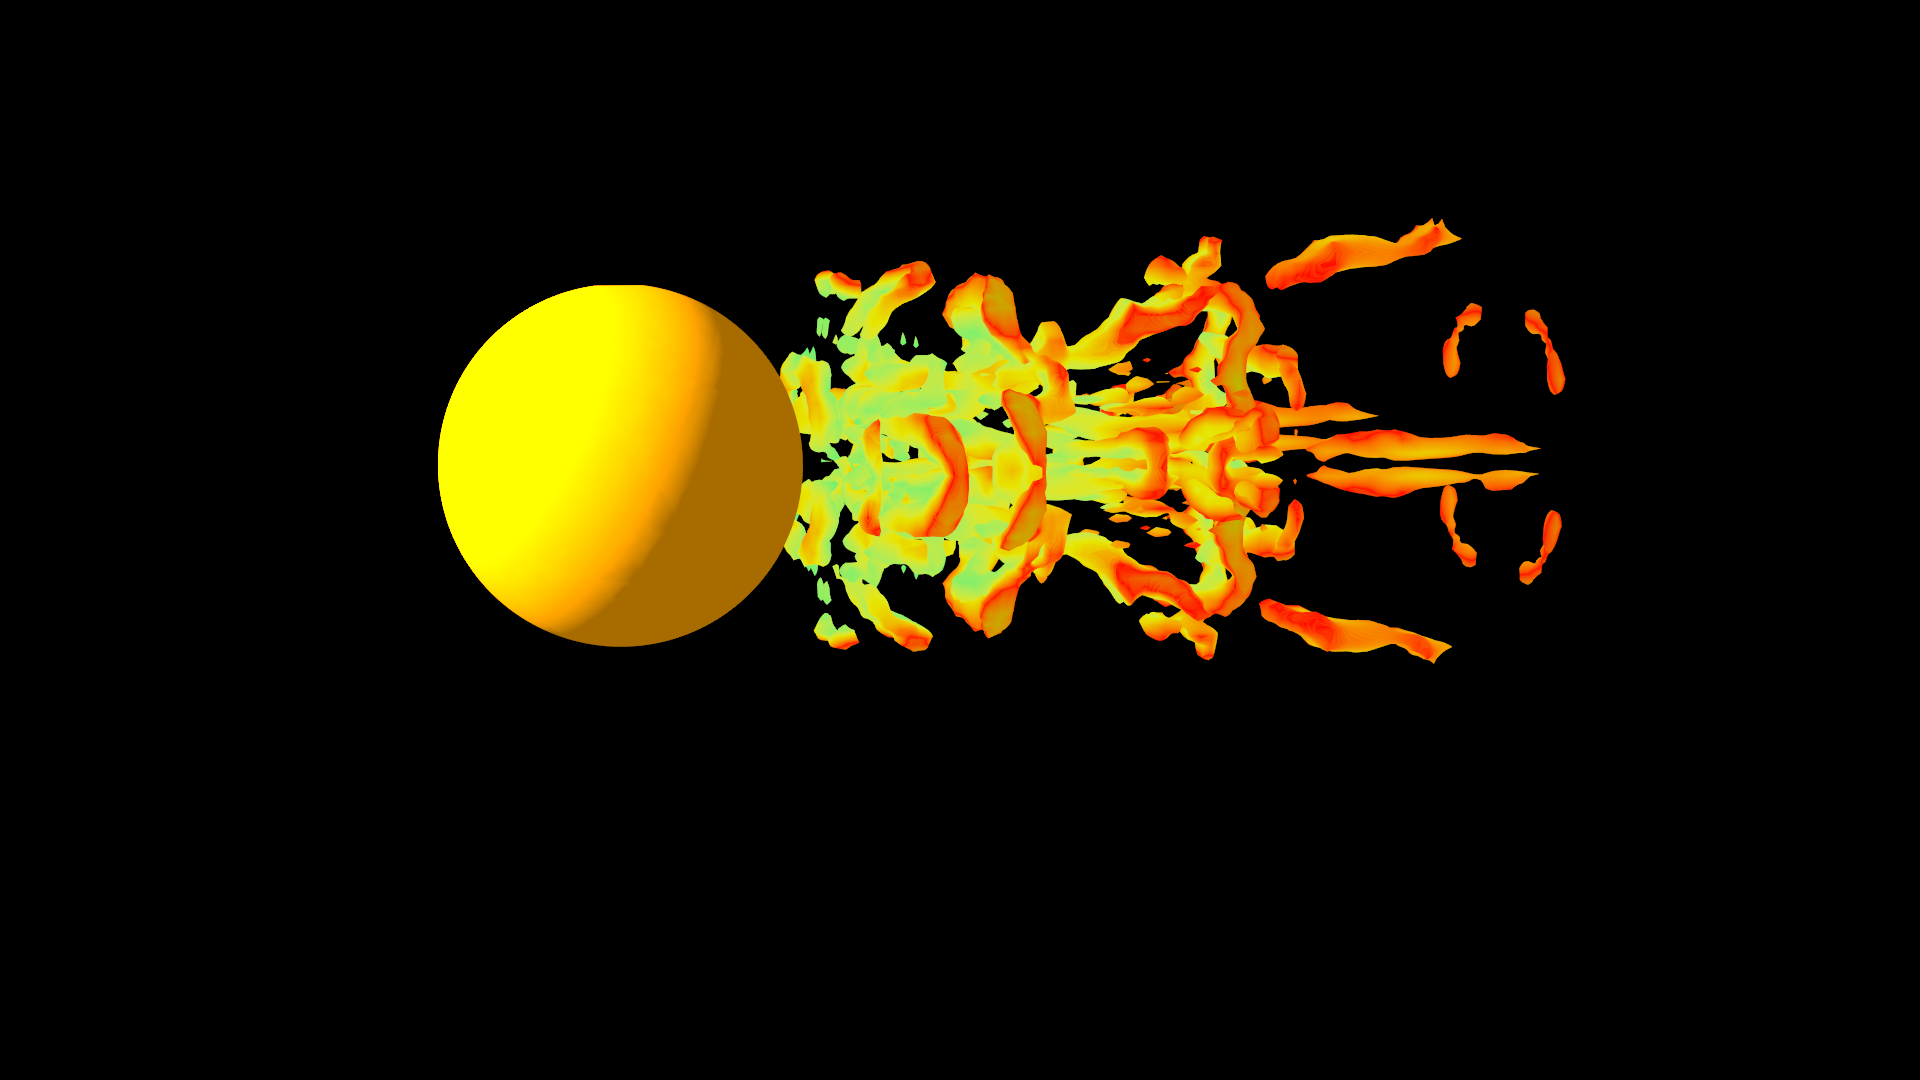
\includegraphics[width=0.45\textwidth]{./image/single_small_1080p_8_filter_4XRES}
        \caption{Single-resolution small field, 1080p resolution, $ \frac{dx}{8} $ step size with object filtering and 4X super resolution anti-aliasing (iso-value = 0.05)}\label{fig:figure15}
    \end{figure}

    \begin{figure}[H]
        \centering
        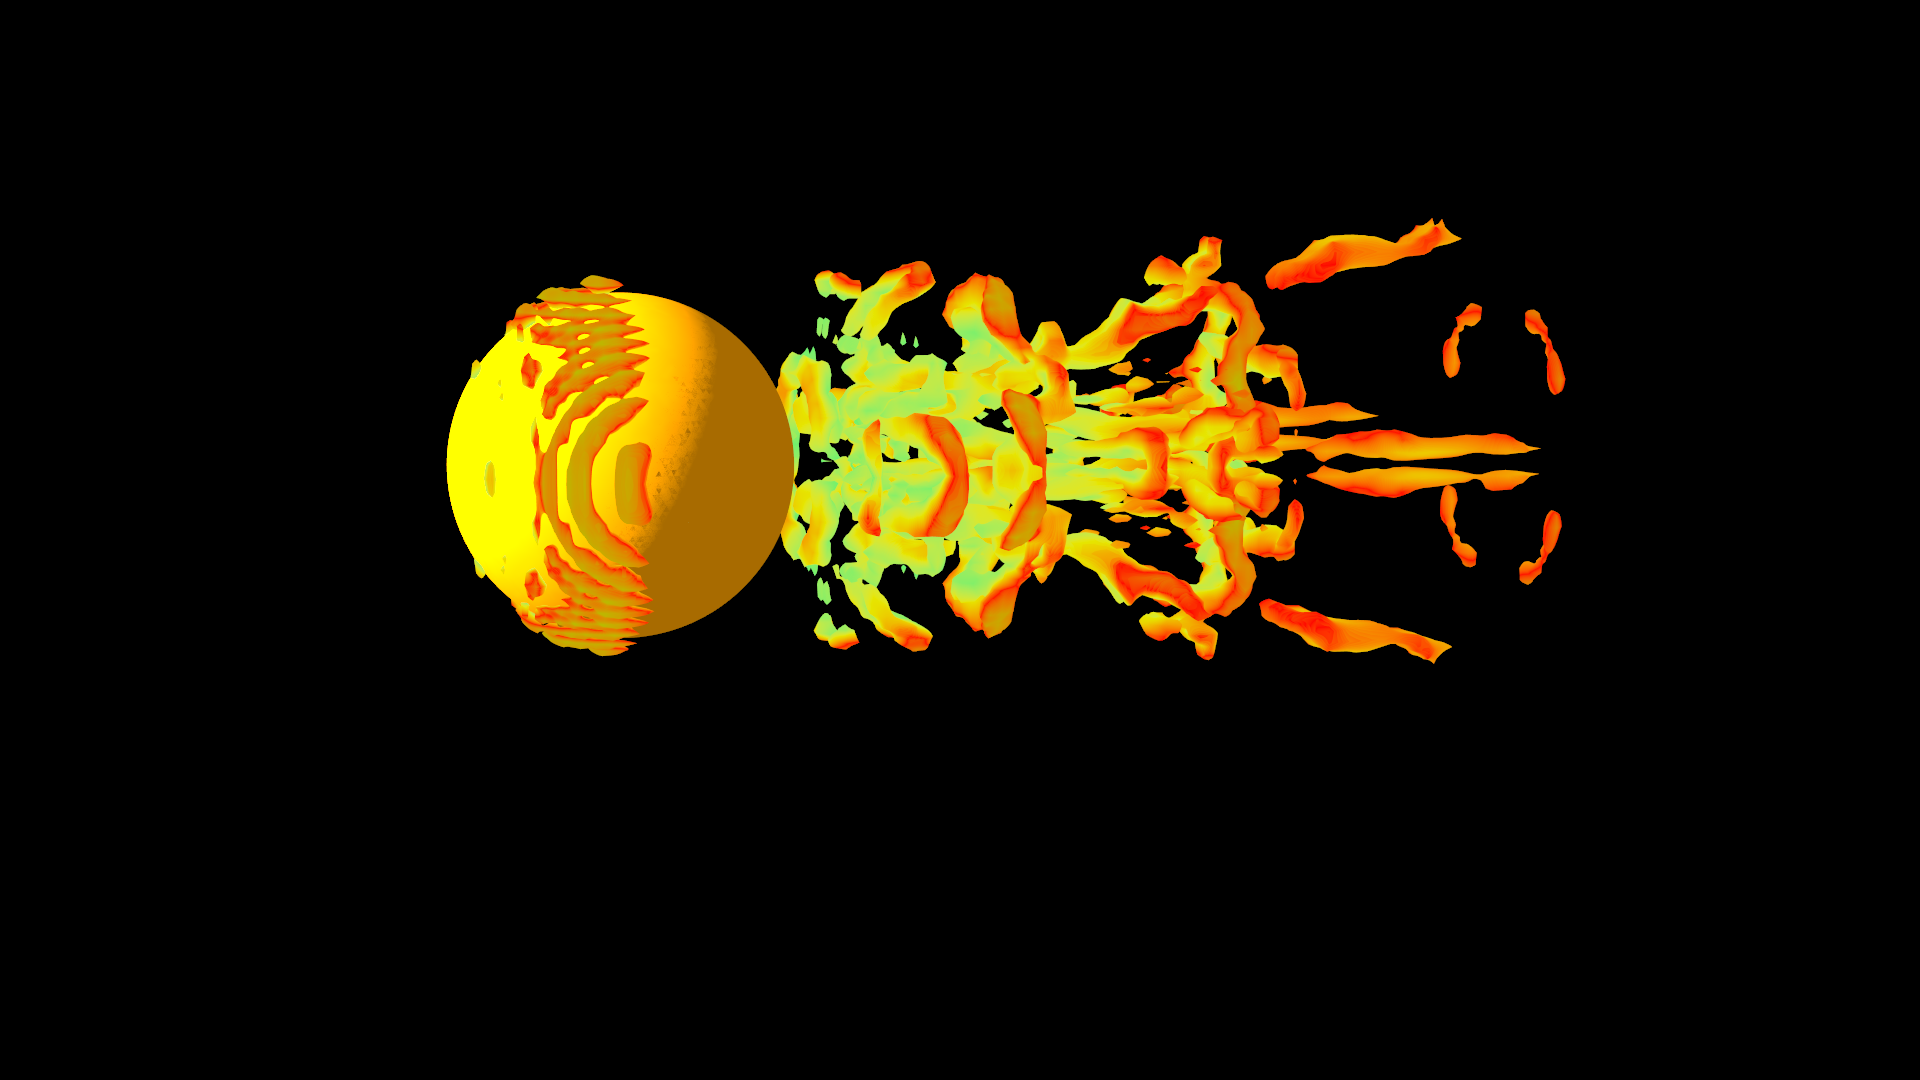
\includegraphics[width=0.45\textwidth]{./image/single_small_1080p_8_no_filter_4XRES}
        \caption{Single-resolution small field, 1080p resolution, $ \frac{dx}{8} $ step size without object filtering and 4X super resolution anti-aliasing (iso-value = 0.05)}\label{fig:figure16}
    \end{figure}

    \section{Division of work}\label{sec:division-of-work}

\end{document}
